\chapter{UJI COBA DAN EVALUASI}\label{chap:uji-coba-eval}

\tab Bab ini membahas skenario uji coba aplikasi yang telah dirancang dan diimplementasikan, serta analisis hasil pengujian. Ada dua jenis pengujian, yakni uji coba fungsionalitas dan uji coba performa. Uji coba dilakukan untuk menganalisis kinerja aplikasi dengan lingkungan uji coba yang telah ditentukan.

\section{Lingkungan Uji Coba}
\tab Lingkungan yang digunakan untuk pengujian meliputi perangkat keras dan
perangkat lunak yang dijelaskan sebagai berikut.

\begin{enumerate}
	\item Perangkat keras (\textit{virtual server}):
	\begin{itemize}
		\item Prosesor Intel(R) Xeon(R) Platinum 8168 CPU @ 2.70GHz (16 VCPUs)
		\item Memori 31 GB
		\item Arsitektur prosesor x86\_64 (64-bit)
	\end{itemize}
	\item Perangkat Lunak:
	\begin{itemize}
		\item Sistem operasi Ubuntu 18.04.2 LTS
		\item Bahasa Pemrograman Python 3.7.3
	\end{itemize}			
\end{enumerate}

\section{Data Uji Coba}

\tab Terdapat tiga jenis data yang akan digunakan dalam pengujian Tugas Akhir ini, yaitu data \textit{independent} (IND), \textit{anti-correlated} (ANT), dan \textit{Forest Cover Type} (FC).

\pagebreak
\subsection{Data \textit{Independent} (IND)}
\tab Data \textit{independent} (IND) adalah himpunan data yang memiliki persebaran nilai atribut yang acak dan tidak saling terpengaruh satu sama lain. Data ini adalah data sintetis yang dibuat untuk menguji performa algoritma jika berhadapan dengan data yang nilai atributnya tidak memiliki keterkaitan satu sama lain. Rentang nilai yang digunakan untuk setiap atribut adalah 1 – 300.

\subsection{Data \textit{Anti-Correlated} (ANT)}
\tab Data \textit{anti-correlated} (ANT) adalah himpunan data yang memiliki
persebaran nilai atribut yang saling bertolak belakang antara satu
atribut dengan atribut lainnya, artinya sebuah data memiliki
nilai yang sangat baik pada salah satu atributnya, namun sangat
buruk pada atribut lainnya. Data ini adalah data sintetis yang dibuat untuk menguji performa algoritma jika berhadapan dengan data yang memiliki banyak titik skyline. Rentang nilai yang digunakan untuk setiap
atribut adalah 1 – 300.

\subsection{Data \textit{Forest Cover Type} (FC)}
\tab Data \textit{Forest Cover Type} (FC) adalah himpunan data asli yang berisi hasil pengamatan pohon dari empat area Hutan Nasional Roosevelt di Colorado. Semua pengamatan adalah variabel kartografi dari 30 meter x 30 meter bagian hutan. Dataset ini mencakup informasi tentang jenis pohon, jangkauan bayangan, jarak ke \textit{landmark} terdekat (jalan dan sebagainya), jenis tanah, dan topografi lokal. \textit{Dataset} ini adalah bagian dari \textit{UCI Machine Learning Repository} yang dikumpulkan oleh Blackard, Dean, dan Anderson (1998) di Colorado \textit{State University} \cite{fc}.

\pagebreak
Himpunan data \textit{Forest Cover Type} (FC) terdiri dari 581.012 data dan memiliki 55 dimensi atribut. Tidak ditemukan nilai yang hilang atau anomali
pada himpunan data ini. Seluruh atribut bertipe data numerik
dengan rincian dapat dilihat pada Tabel \ref{tab:atribut-fc}.

\begin{table}[H]
	\centering
	\begin{tabular}{ | p{6cm} | p{1cm} | }
		\hline
		\multicolumn{1}{|c}{\textbf{Nama Kolom}} & \multicolumn{1}{|c|}{\textbf{Jumlah Kolom}} \\ \hline \hline
		Elevation & 1 \\ \hline
		Aspect & 1 \\ \hline
		Slope & 1  \\ \hline
		Horizontal\_Distance\_To\_Hydrology & 1 \\ \hline 
		Vertical\_Distance\_To\_Hydrology & 1 \\ \hline 
		Horizontal\_Distance\_To\_Roadways & 1 \\ \hline
		Hillshade\_9am & 1 \\ \hline
		Hillshade\_Noon & 1 \\ \hline
		Hillshade\_3pm & 1 \\ \hline
		Horizontal\_Distance\_To\_Fire\_Points & 1 \\ \hline
		Wilderness\_Area & 4 \\ \hline
		Soil\_Type & 40 \\ \hline
		Cover\_Type & 1 \\ \hline
	\end{tabular} \caption{Atribut himpunan data \textit{Forest Cover Type}}
	\label{tab:atribut-fc}
\end{table}

Data \textit{Forest Cover Type} (FC) adalah himpunan data yang
diambil dari sumber sebenarnya. Penggunaan data ini bertujuan
untuk menguji performa algoritma pada data dengan persebaran
dan rentang nilai atribut sebenarnya yang bersifat saling berkaitan.

\pagebreak
\section{Skenario Uji Coba} \label{skenarioujicoba}
\tab Uji coba ini dilakukan untuk menguji apakah program yang telah diimplementasikan dapat berjalan dengan sebagaimana mestinya. Uji coba akan dibagi menjadi dua jenis, yaitu uji coba fungsionalitas dan uji coba performa.

\subsection{Uji Coba Fungsionalitas}
\tab Skenario uji coba fungsionalitas berfokus pada pengujian apakah aplikasi dapat digunakan sesuai dengan kebutuhan fungsional pada Tabel \ref{tab:kebutuhan-fungsional}. Skenario pengujian fungsionalitas aplikasi ditunjukkan pada Tabel \ref{tab:uji-coba-fungsional}.

\begin{table}[H]
	\centering
	\begin{tabular}{ | c | p{8cm} | }
		\hline
		\multicolumn{1}{|c}{\textbf{No.}} & \multicolumn{1}{|c|}{\textbf{Deskripsi Kebutuhan}} \\ \hline \hline
		1 & Pengguna dapat mengunggah data \\ \hline
		2 & Pengguna dapat melihat informasi dan pratinjau data \\ \hline
		3 & Pengguna dapat melihat visualisasi data  \\ \hline
		4 & Pengguna dapat memilih algoritme yang digunakan untuk \textit{data precomputing}\\ \hline
		5 & Pengguna dapat memasukkan kueri pencarian \\ \hline
		6 & Pengguna dapat melihat hasil kueri \\ \hline
	\end{tabular} \caption{Skenario uji coba fungsionalitas}
	\label{tab:uji-coba-fungsional}
\end{table}

\subsection{Uji Coba Performa}
\tab Pengujian performa bertujuan untuk membandingkan kinerja masing-masing algoritme dalam melakukan \textit{data precomputing}. Dalam sebuah percobaan atau pengujian, biasanya dikenal adanya tiga jenis variabel, yaitu variabel kontrol, manipulasi, dan respon. 

\pagebreak
Variabel kontrol adalah variabel yang dikendalikan, biasanya dibuat konstan sehingga pengaruh variabel manipulasi terhadap variabel respon tidak dipengaruhi oleh faktor luar yang tidak diteliti. Variabel manipulasi adalah variabel yang dapat memicu suatu perubahan bagi variabel respon. Variabel respon adalah variabel yang berubah akibat dari variabel manipulasi.

Dalam pengujian ini, variabel kontrol yang digunakan adalah jenis data dan jenis algoritme, variabel manipulasinya adalah jumlah data dan jumlah dimensi data, sedangkan variabel responnya berupa waktu komputasi dan penggunaan memori. Skenario pengujian performa ditunjukkan pada Tabel \ref{tab:uji-coba-performa-precompute}.

\begin{longtable}{| c | p{3cm} | p{1cm} | p{2.5cm} | p{1.5cm} |}
	\caption{Skenario uji coba performa \textit{data precomputing} \label{tab:uji-coba-performa-precompute}}\\
	\hline
	\textbf{No.} & \textbf{Jenis Algoritme} & \textbf{Jenis Data} & \textbf{Jumlah Data ($n$)} & \textbf{Jumlah Dimensi ($d$)} \\ \hline
	\endfirsthead
	\hline
	\textbf{No.} & \textbf{Jenis Algoritme} & \textbf{Jenis Data} & \textbf{Jumlah Data ($n$)} & \textbf{Jumlah Dimensi ($d$)} \\ \hline
	\endhead
	\multirow{3}{*}{1} & k-MPPTI & \multirow{3}{1cm}{IND} & \multirow{3}{2.5cm}{100, 500, 1000, 5000, 10000} & \multirow{3}{1.5cm}{3} \\ \cline{2-2} \nopagebreak
	& k-MPPTI Paralel & & & \\ \cline{2-2} \nopagebreak
	& k-MPPTI NoRSL & & & \\ \hline
	\multirow{3}{*}{2} & k-MPPTI & \multirow{3}{1cm}{ANT} & \multirow{3}{2.5cm}{100, 500, 1000, 5000, 10000} & \multirow{3}{1.5cm}{3}\\ \cline{2-2} \nopagebreak
	& k-MPPTI Paralel & & & \\ \cline{2-2} \nopagebreak
	& k-MPPTI NoRSL & & & \\ \hline
	\multirow{3}{*}{3} & k-MPPTI & \multirow{3}{1cm}{FC} & \multirow{3}{2.5cm}{100, 500, 1000, 5000, 10000} & \multirow{3}{1.5cm}{3}\\ \cline{2-2} \nopagebreak
	& k-MPPTI Paralel & & & \\ \cline{2-2} \nopagebreak
	& k-MPPTI NoRSL & & & \\ \hline 
	\multirow{3}{*}{4} & k-MPPTI & \multirow{3}{1cm}{IND} & \multirow{3}{2.5cm}{1000} & \multirow{3}{1.5cm}{2, 3, 5, 7, 10}\\ \cline{2-2}	\nopagebreak	
	& k-MPPTI Paralel & & & \\ \cline{2-2} \nopagebreak
	& k-MPPTI NoRSL & & & \\ \hline \pagebreak
	\multirow{3}{*}{5} & k-MPPTI & \multirow{3}{1cm}{ANT} & \multirow{3}{2.5cm}{1000} & \multirow{3}{1.5cm}{2, 3, 5, 7, 10}\\ \cline{2-2}\nopagebreak
	& k-MPPTI Paralel & & & \\ \cline{2-2} \nopagebreak
	& k-MPPTI NoRSL & & & \\ \hline 
	\multirow{3}{*}{6} & k-MPPTI & \multirow{3}{1cm}{FC} & \multirow{3}{2.5cm}{1000} & \multirow{3}{1.5cm}{2, 3, 5, 7, 10}\\ \cline{2-2} \nopagebreak
	& k-MPPTI Paralel & & & \\ \cline{2-2} \nopagebreak
	& k-MPPTI NoRSL & & & \\ \hline
\end{longtable}

\section{Analisis Hasil Uji Coba}
\tab Setelah pengujian dilakukan, selanjutnya adalah menganalisis hasil uji coba. Analisis hasil uji coba dibagi menjadi dua bagian, yaitu hasil uji coba fungsionalitas dan hasil uji coba performa.

\subsection{Uji Coba Fungsionalitas}
\tab Pengujian fungsionalitas dilakukan sesuai dengan skenario daftar kebutuhan fungsional pada Tabel \ref{tab:uji-coba-fungsional} yang hasilnya dapat dilihat pada Tabel \ref{tab:hasil-uji-coba-fungsional}. 

Berdasarkan hasil uji coba, aplikasi dapat memenuhi semua kebutuhan fungsional, yakni mengunggah data (Gambar \ref{fig:hasil-performa1}), melihat informasi (Gambar \ref{fig:hasil-performa3}) dan pratinjau data (Gambar \ref{fig:hasil-performa4}), melihat visualisasi data dalam bentuk lini masa (Gambar \ref{fig:hasil-performa5}), memilih algoritme untuk \textit{data precomputing} (Gambar \ref{fig:hasil-performa1}), memasukkan kueri pencarian (Gambar \ref{fig:hasil-performa6}), dan melihat hasil kueri (Gambar \ref{fig:hasil-performa6}).

\begin{table}[H]
	\centering
	\begin{tabular}{ | c | p{5cm} | p{2cm} | }
		\hline
		\multicolumn{1}{|c}{\textbf{No.}} & \multicolumn{1}{|c}{\textbf{Deskripsi Kebutuhan}} & \multicolumn{1}{|c|}{\textbf{Status}}\\ \hline \hline
		1 & Pengguna dapat mengunggah data & Berhasil\\ \hline
		2 & Pengguna dapat melihat informasi dan pratinjau data & Berhasil\\ \hline
		3 & Pengguna dapat melihat visualisasi data & Berhasil \\ \hline
		4 & Pengguna dapat memilih algoritme yang digunakan untuk \textit{data precomputing} & Berhasil\\ \hline
		5 & Pengguna dapat memasukkan kueri pencarian & Berhasil \\ \hline
		6 & Pengguna dapat melihat hasil kueri & Berhasil\\ \hline
	\end{tabular} \caption{Hasil uji coba fungsionalitas}
	\label{tab:hasil-uji-coba-fungsional}
\end{table}

Sebagai tambahan, aplikasi juga memiliki fitur \textit{session} (Gambar \ref{fig:hasil-performa7}) supaya pengguna dapat melakukan dua kali proses \textit{data precomputing} menggunakan data yang berbeda tanpa saling menumpuk satu sama lain. Pengguna hanya perlu memilih \textit{session} yang diinginkan, kemudian melakukan kueri pencarian atau melihat visualisasi data. \\

\begin{figure}[H]
	\centering
	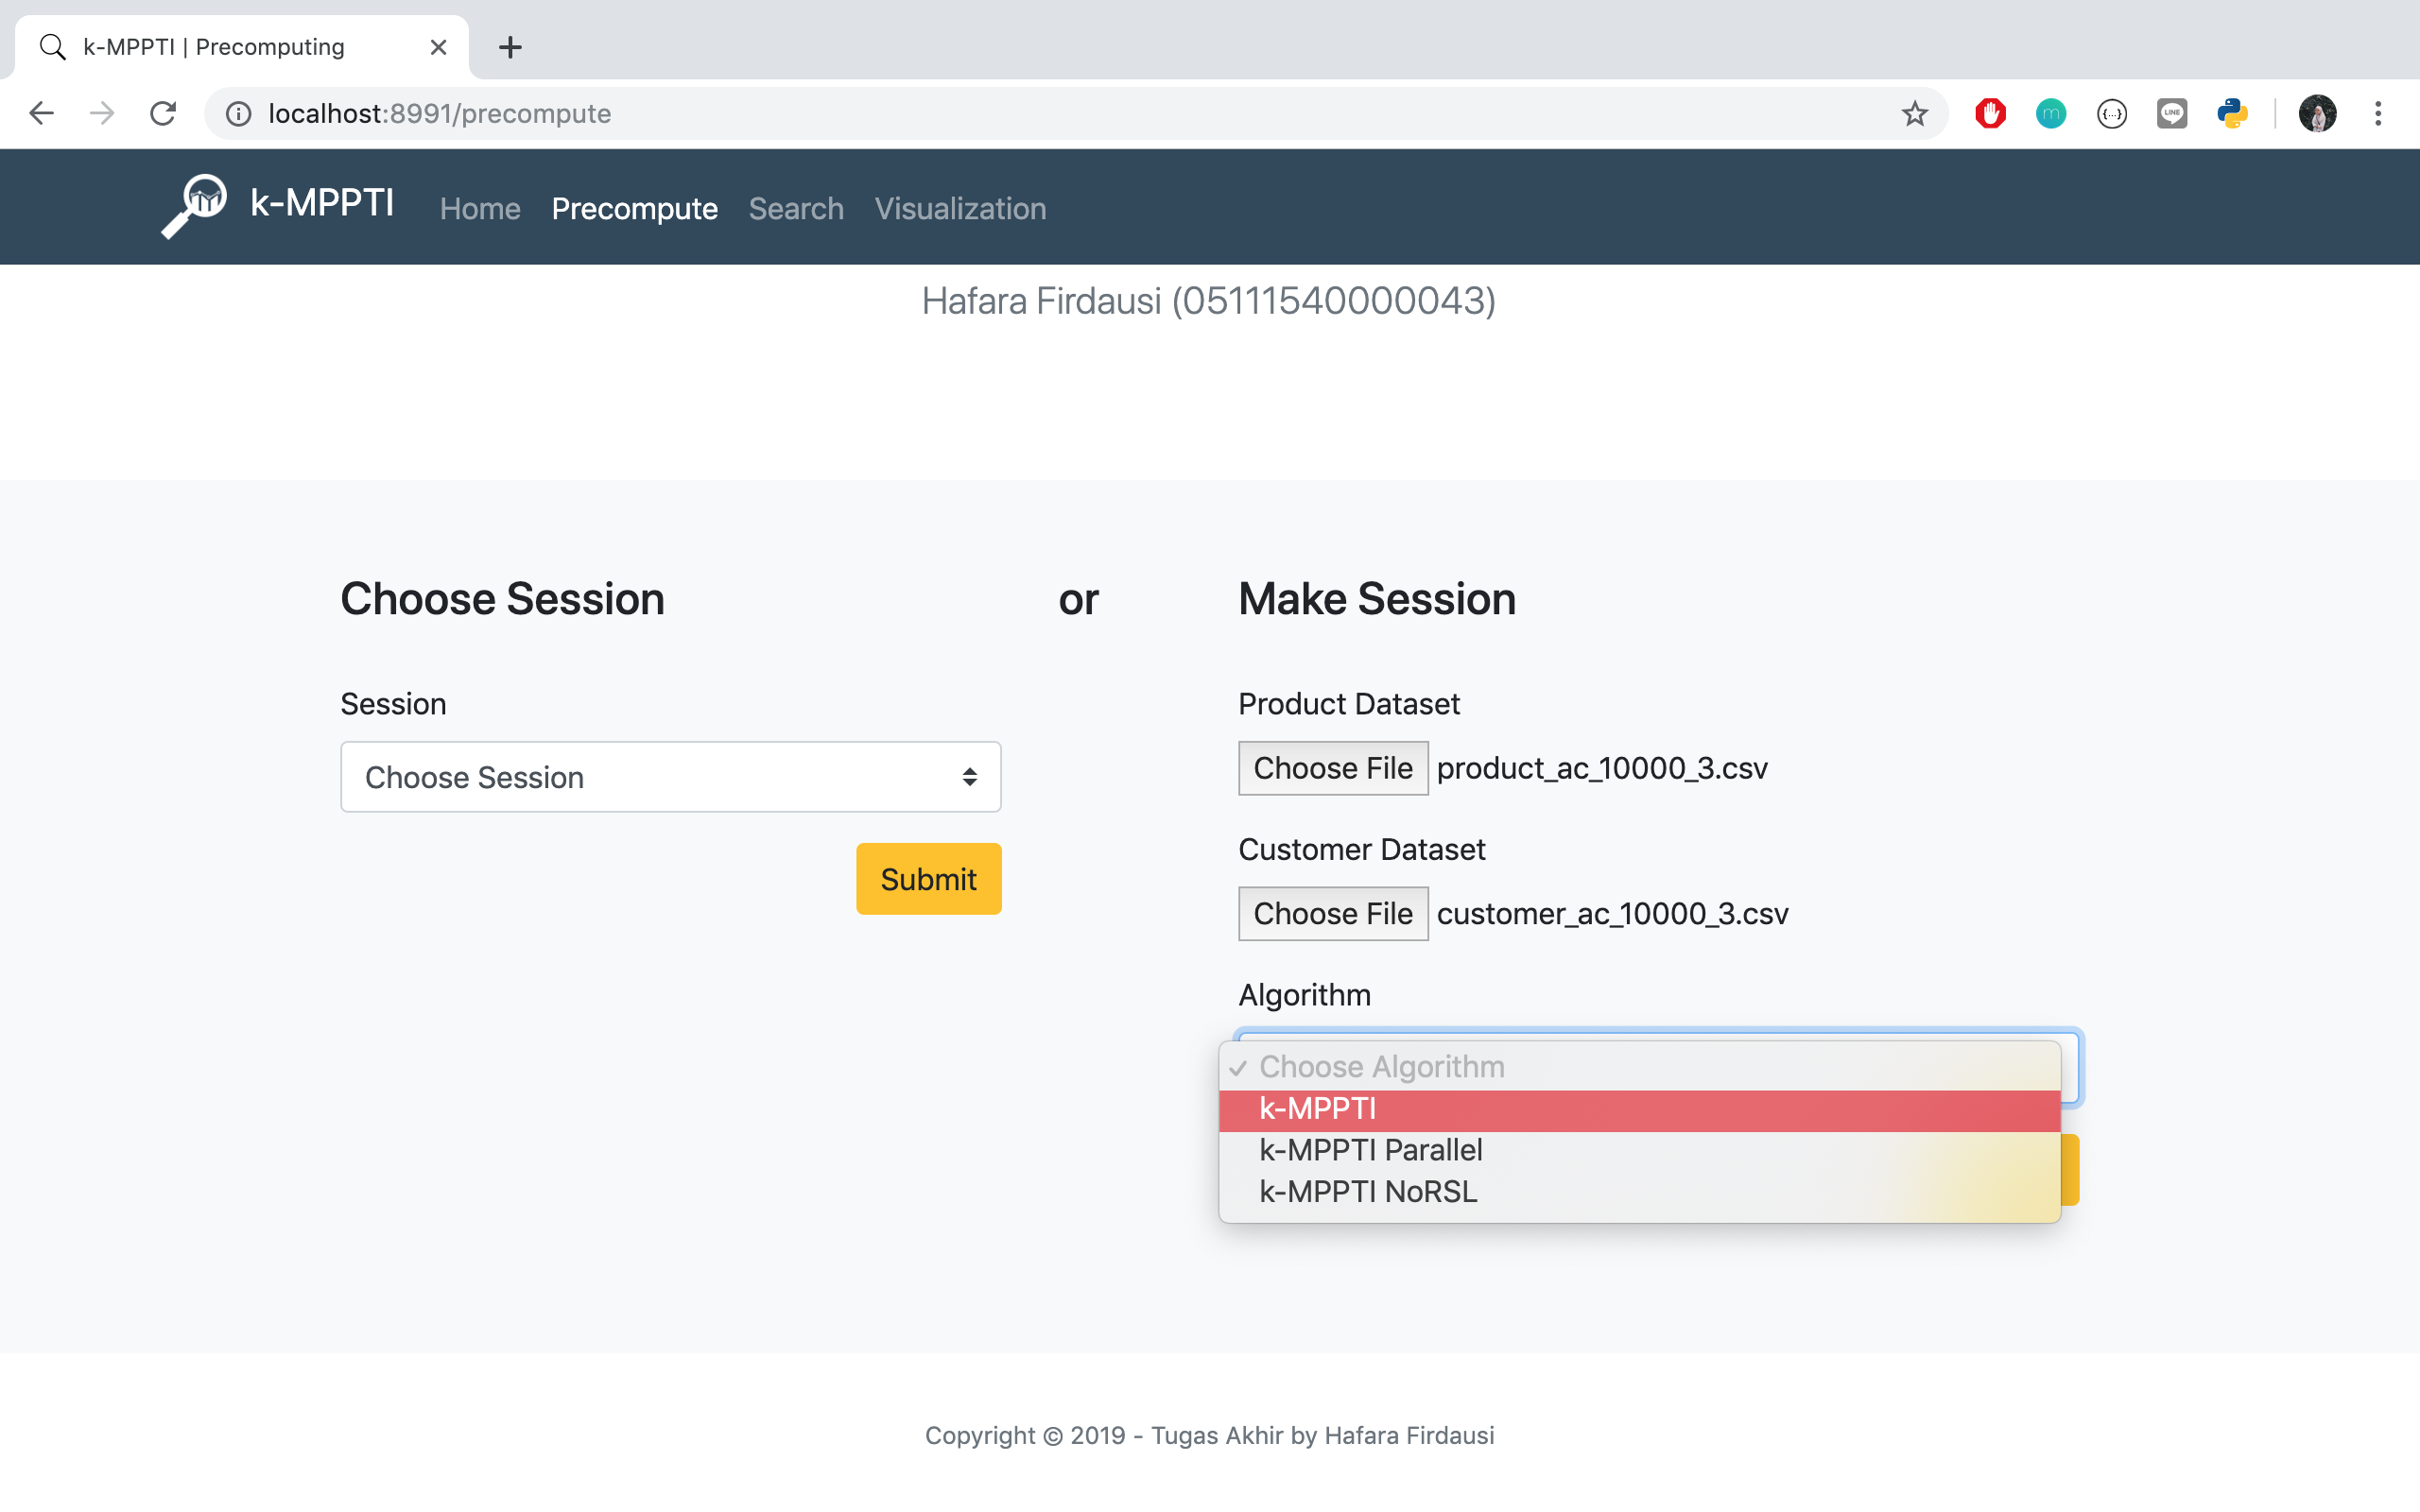
\includegraphics[width=10cm]{assets/img/bab5/hasil2.png}
	\caption{Hasil uji coba: mengunggah data dan memilih algoritme untuk \textit{data precomputing}}
	\label{fig:hasil-performa1}
\end{figure}

\begin{figure}[H]
	\centering
	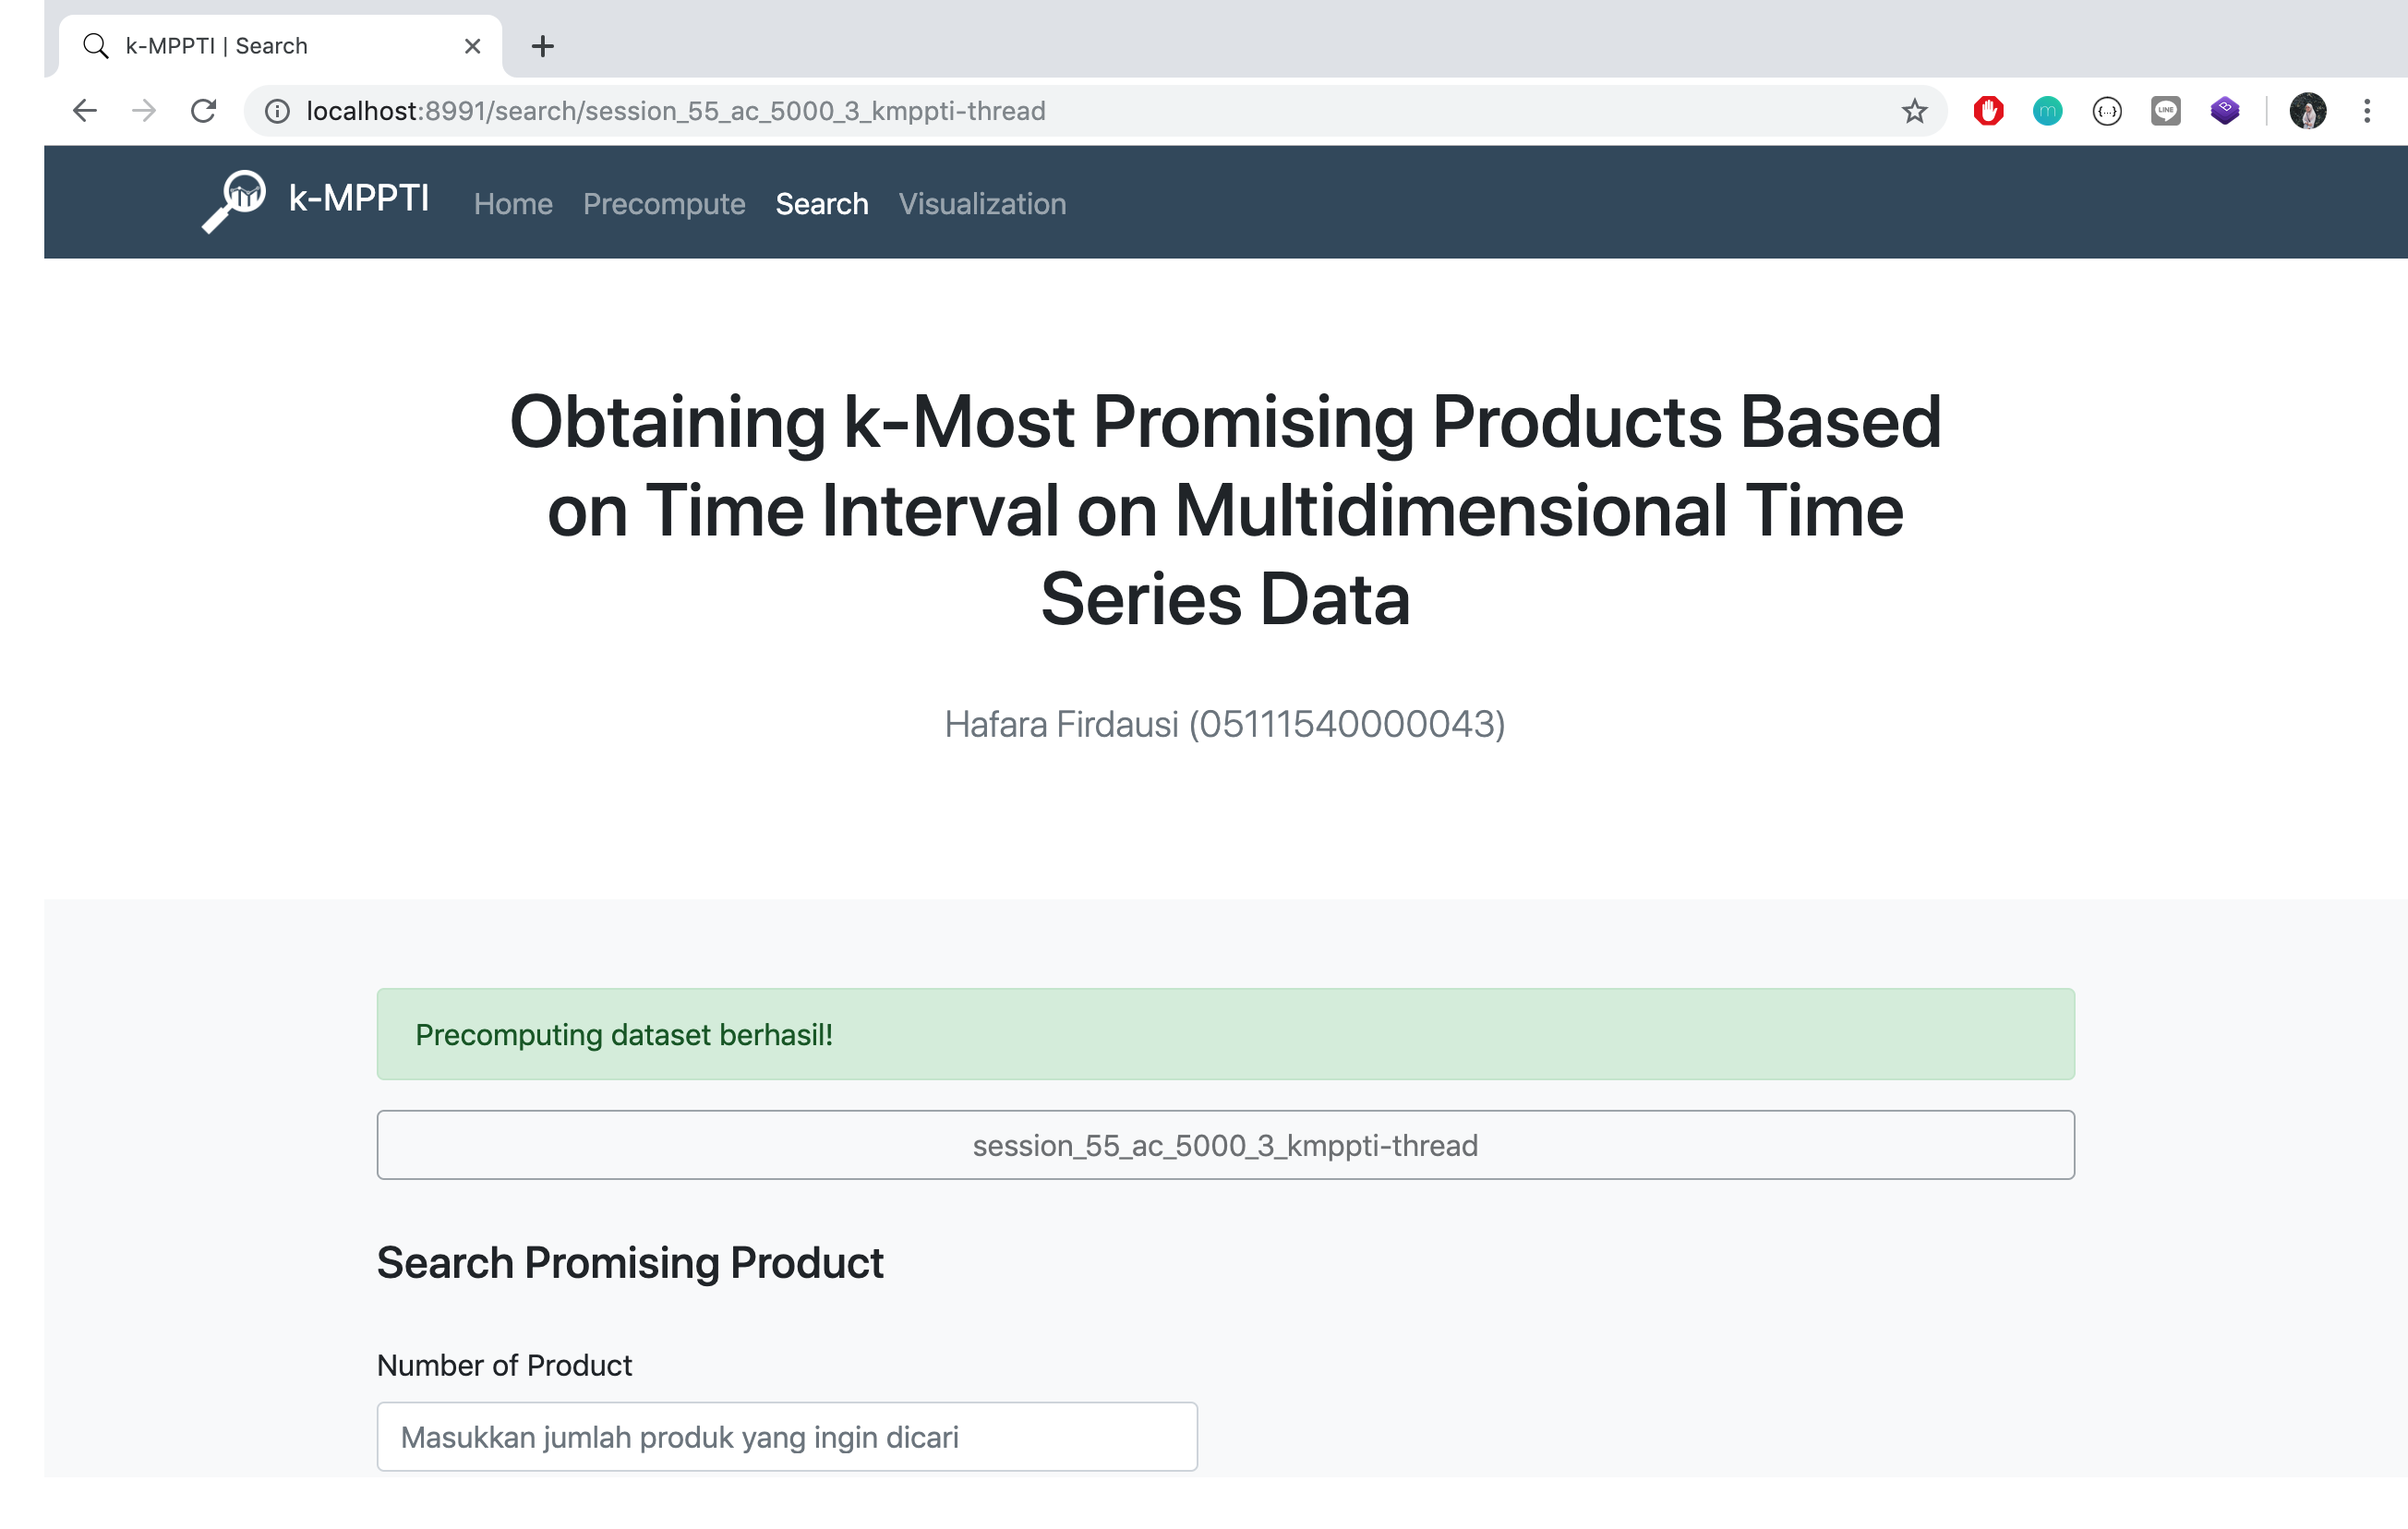
\includegraphics[width=10cm]{assets/img/bab5/hasil1.png}
	\caption{Hasil uji coba: proses \textit{data precomputing} berhasil}
	\label{fig:hasil-performa2}
\end{figure}

\begin{figure}[H]
	\centering
	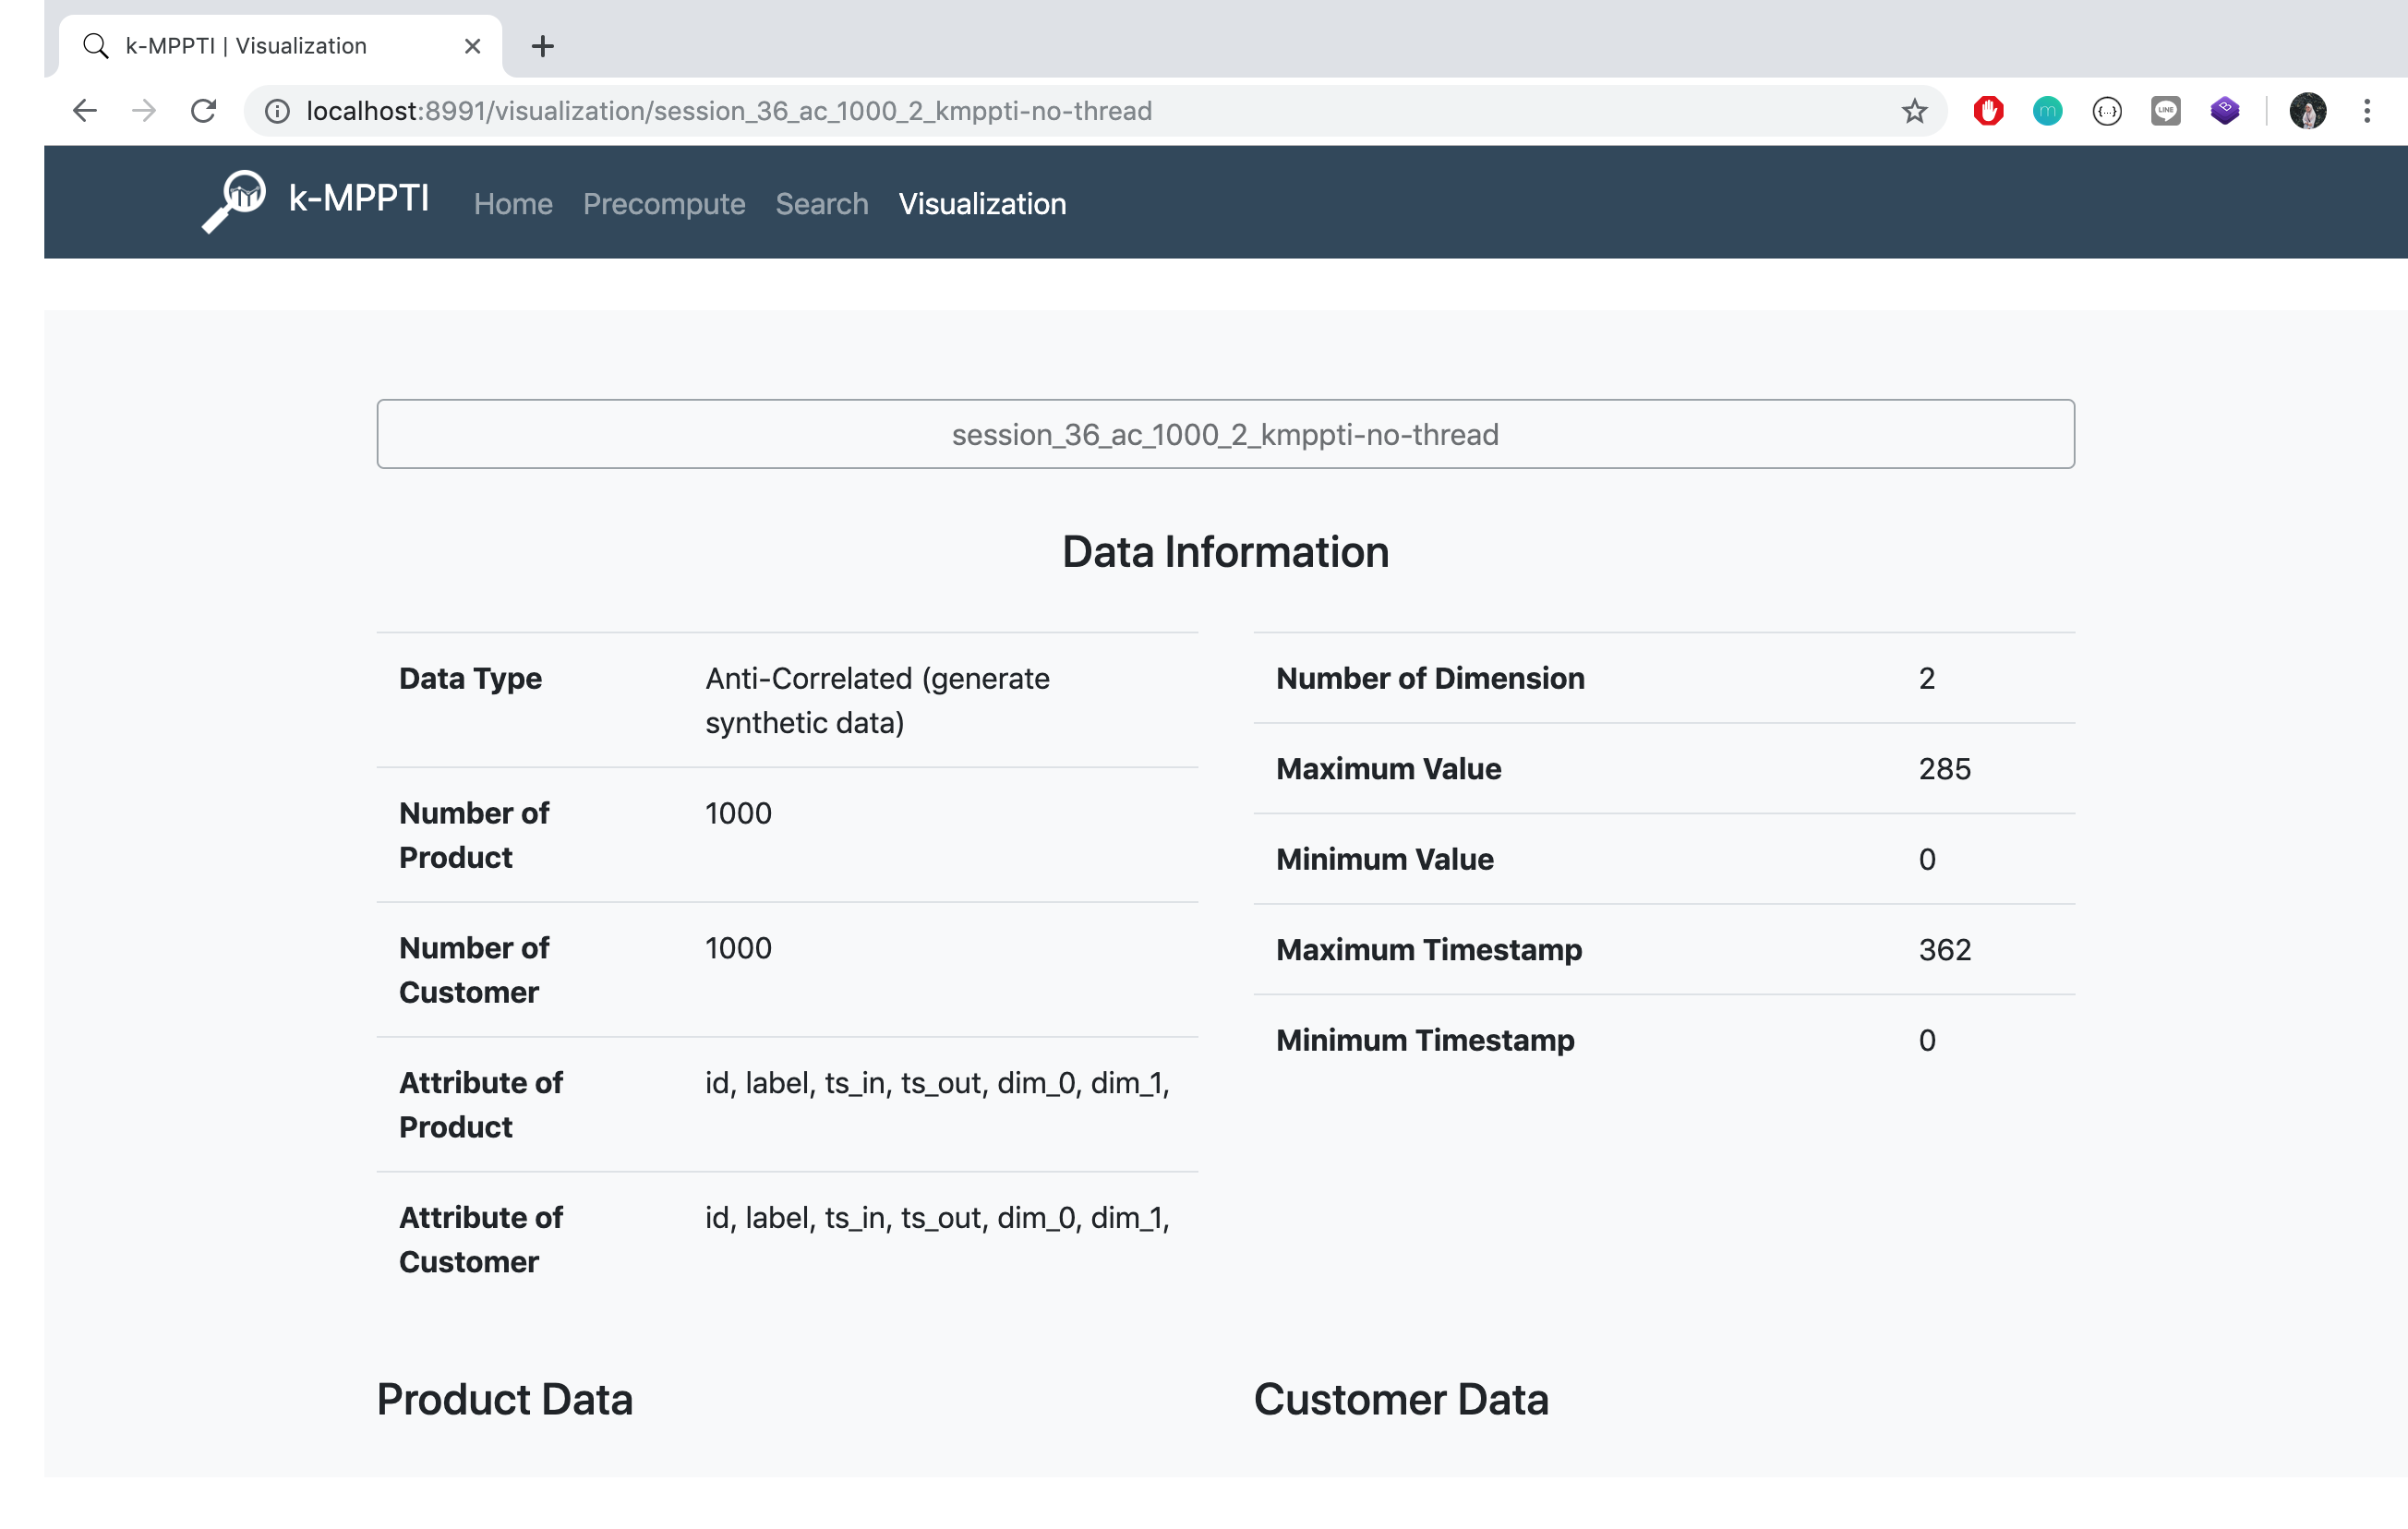
\includegraphics[width=10cm]{assets/img/bab5/hasil3.png}
	\caption{Hasil uji coba: melihat informasi data}
	\label{fig:hasil-performa3}
\end{figure}

\begin{figure}[H]
	\centering
	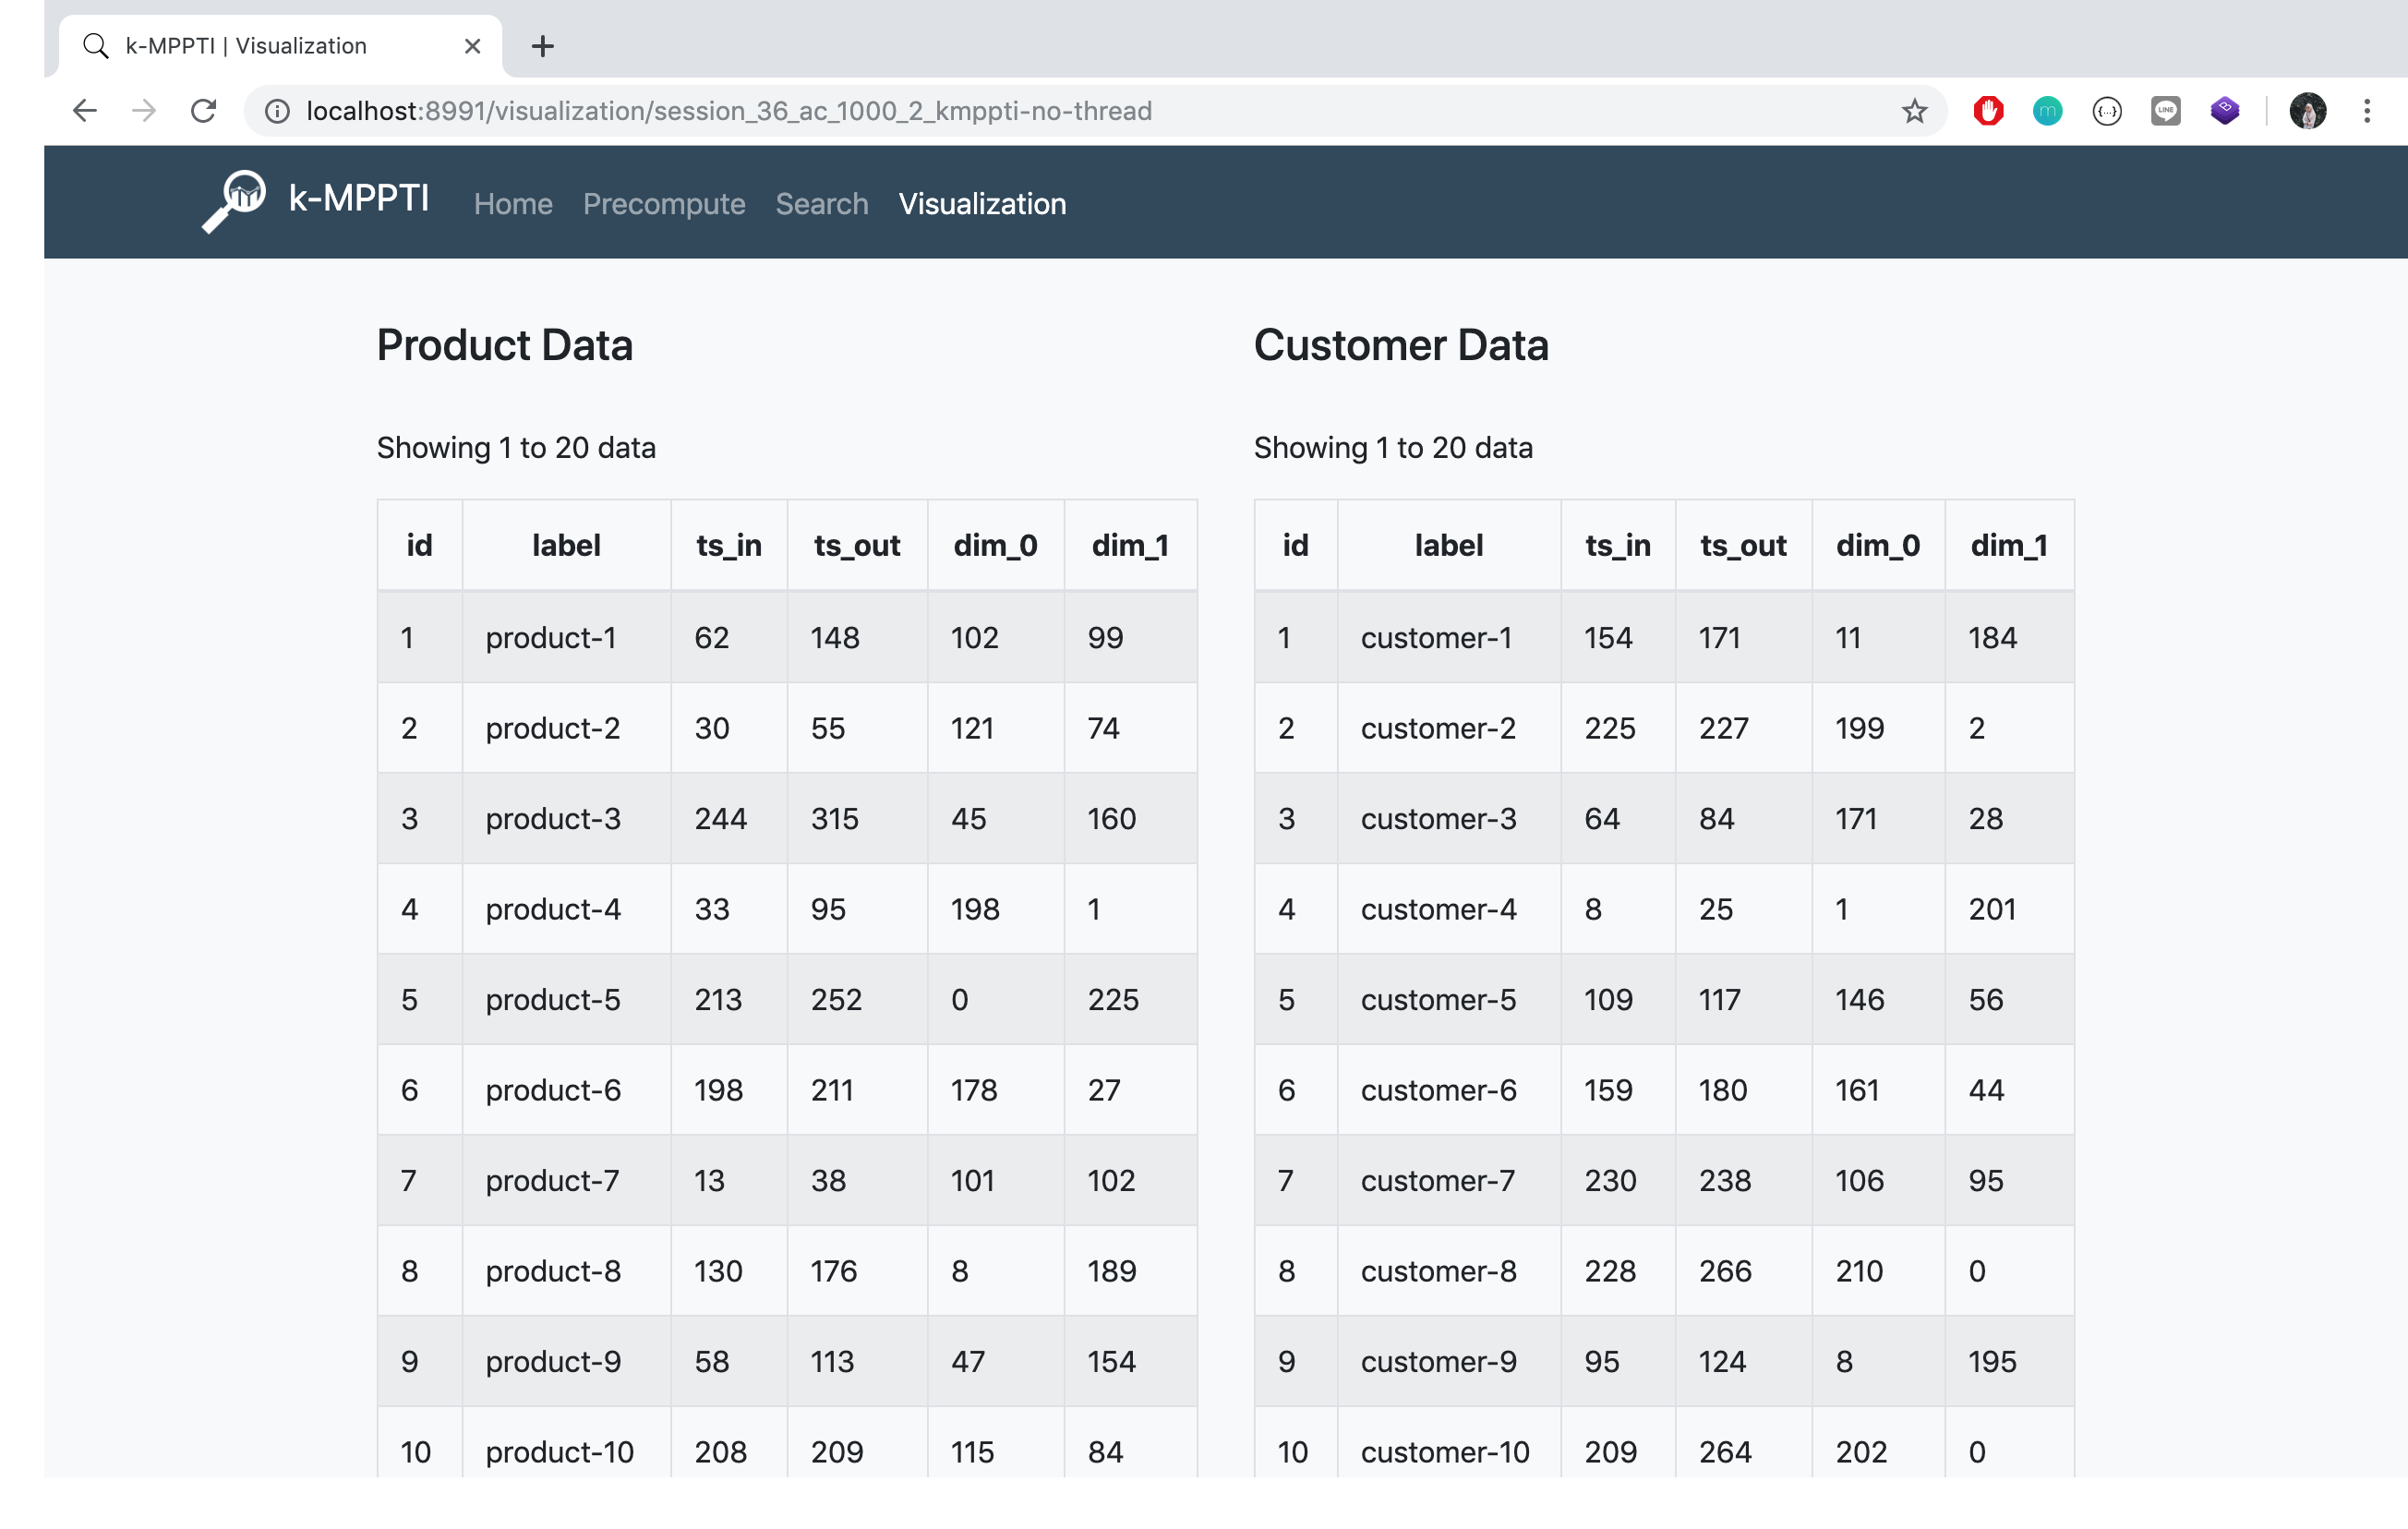
\includegraphics[width=10cm]{assets/img/bab5/hasil4.png}
	\caption{Hasil uji coba: melihat pratinjau data berupa tabel}
	\label{fig:hasil-performa4}
\end{figure}

\begin{figure}[H]
	\centering
	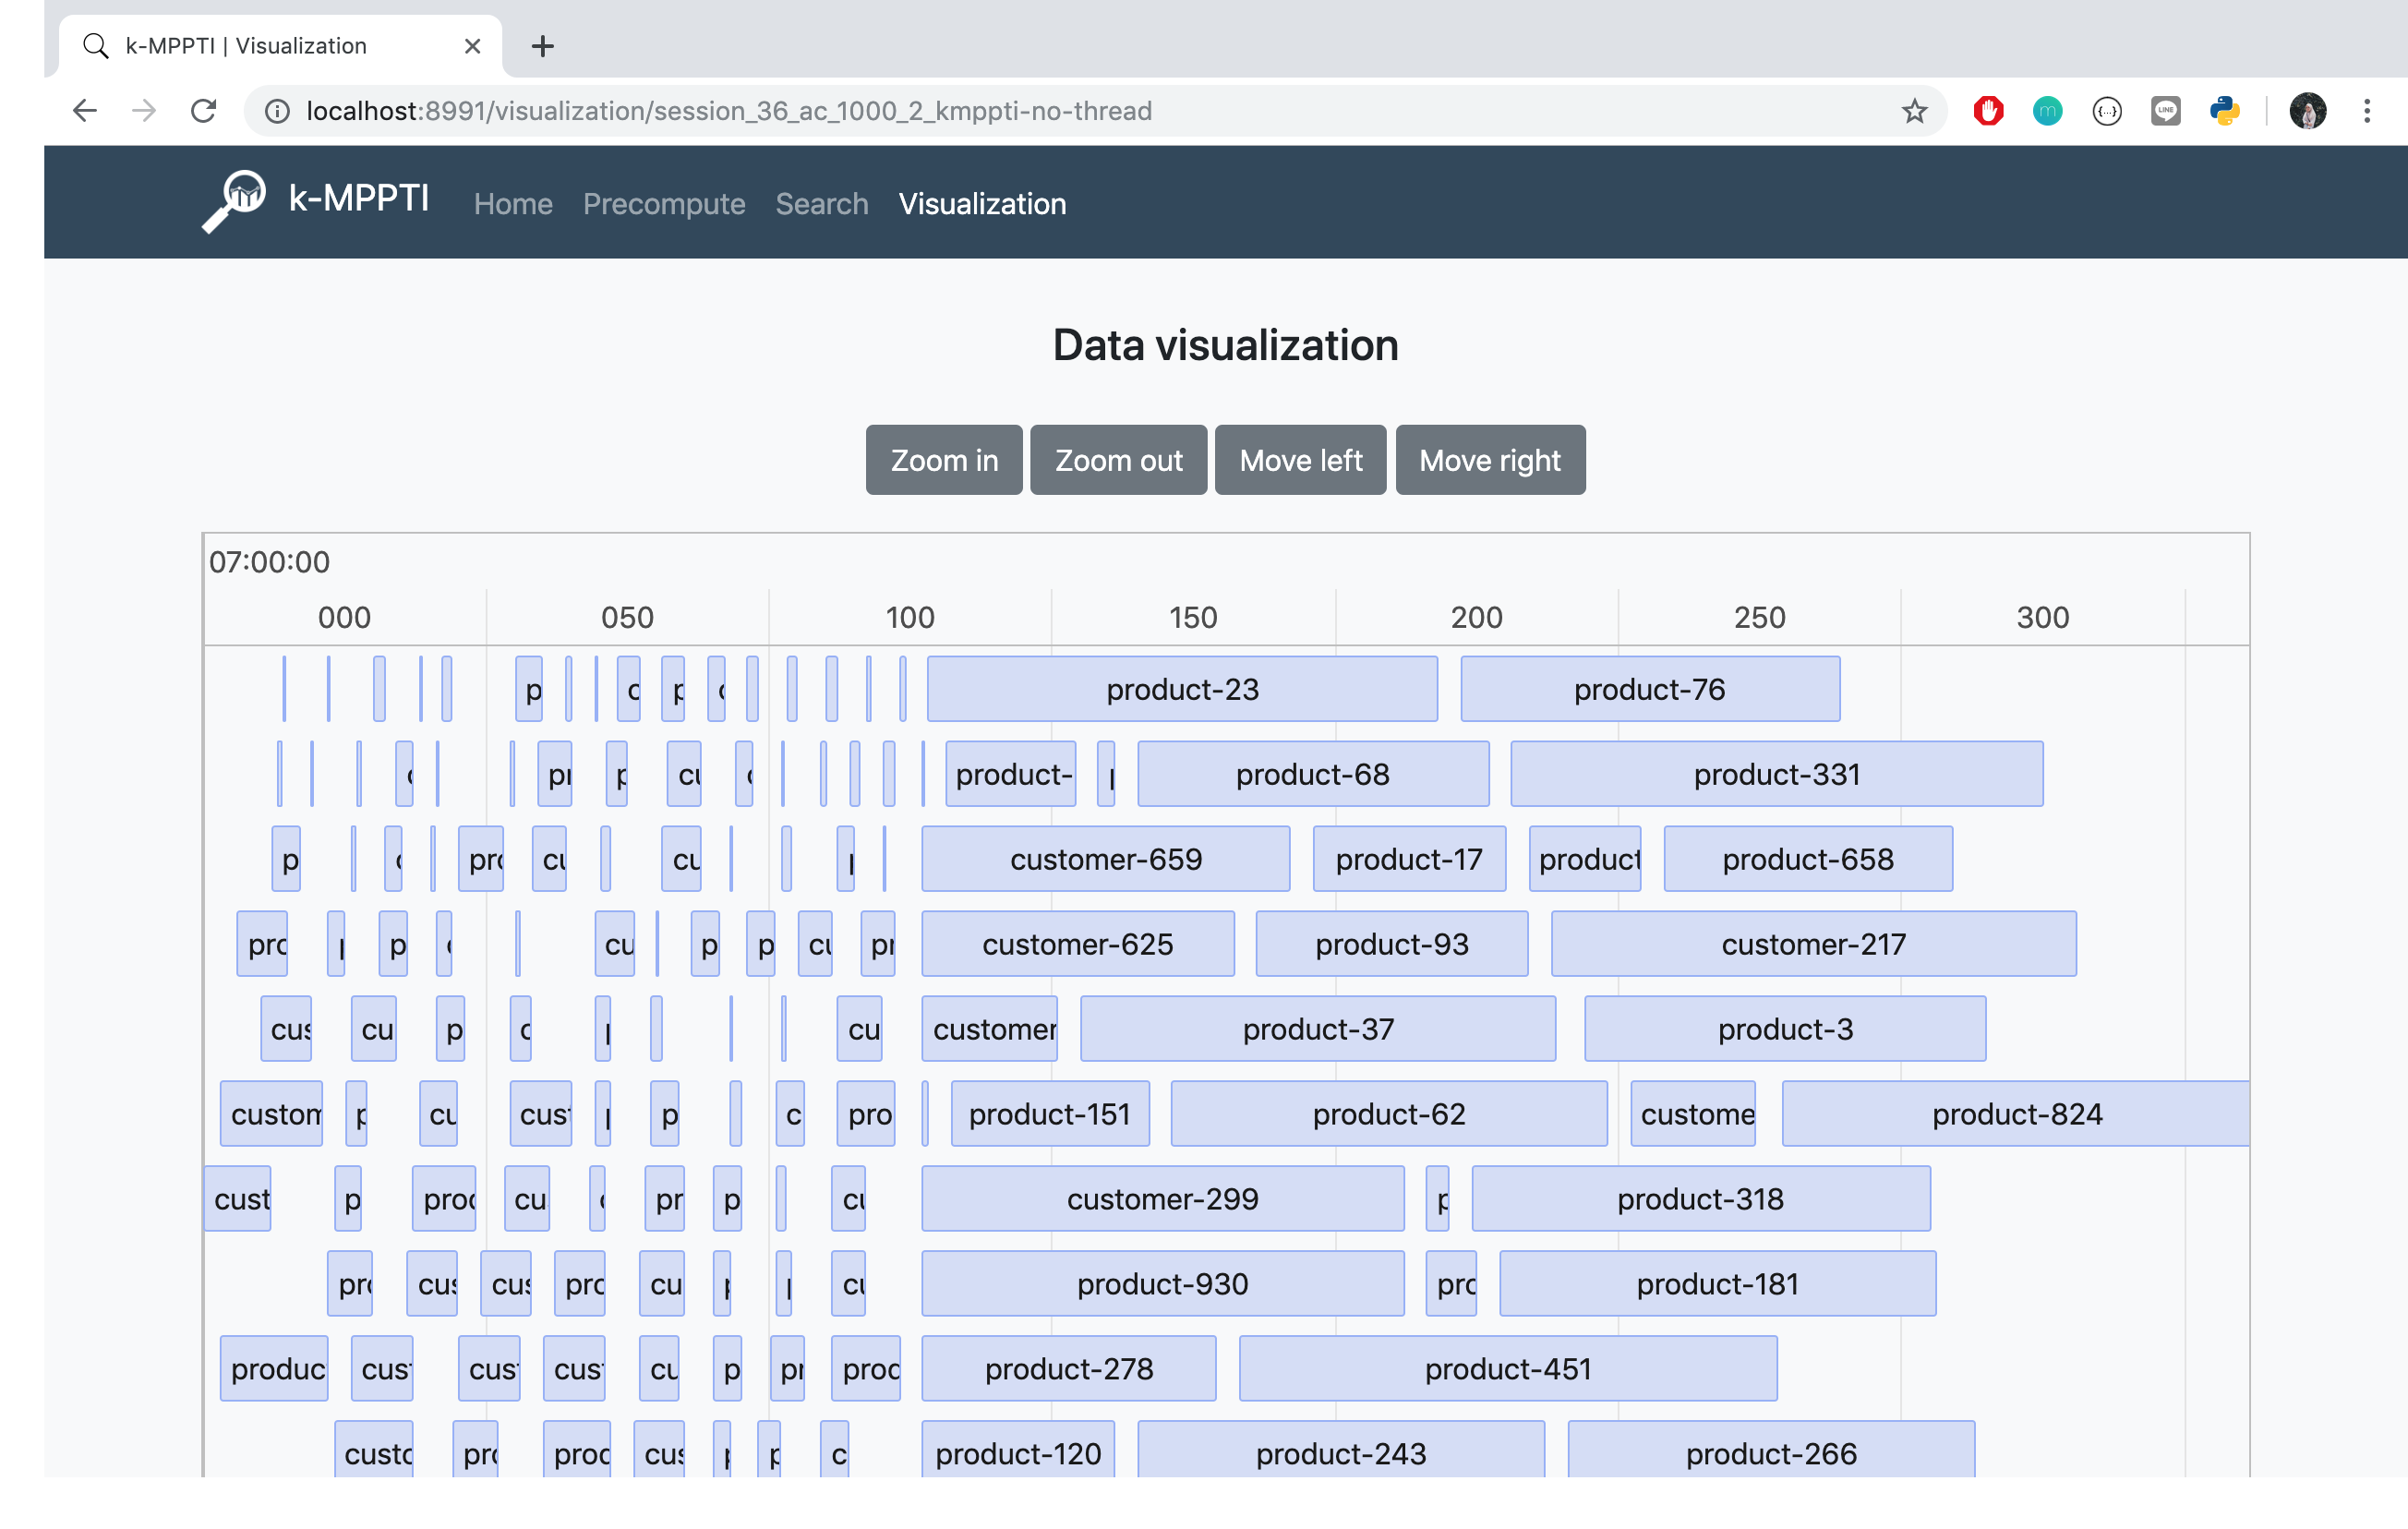
\includegraphics[width=10cm]{assets/img/bab5/hasil5.png}
	\caption{Hasil uji coba: melihat visualisasi data berupa lini masa}
	\label{fig:hasil-performa5}
\end{figure}

\begin{figure}[H]
	\centering
	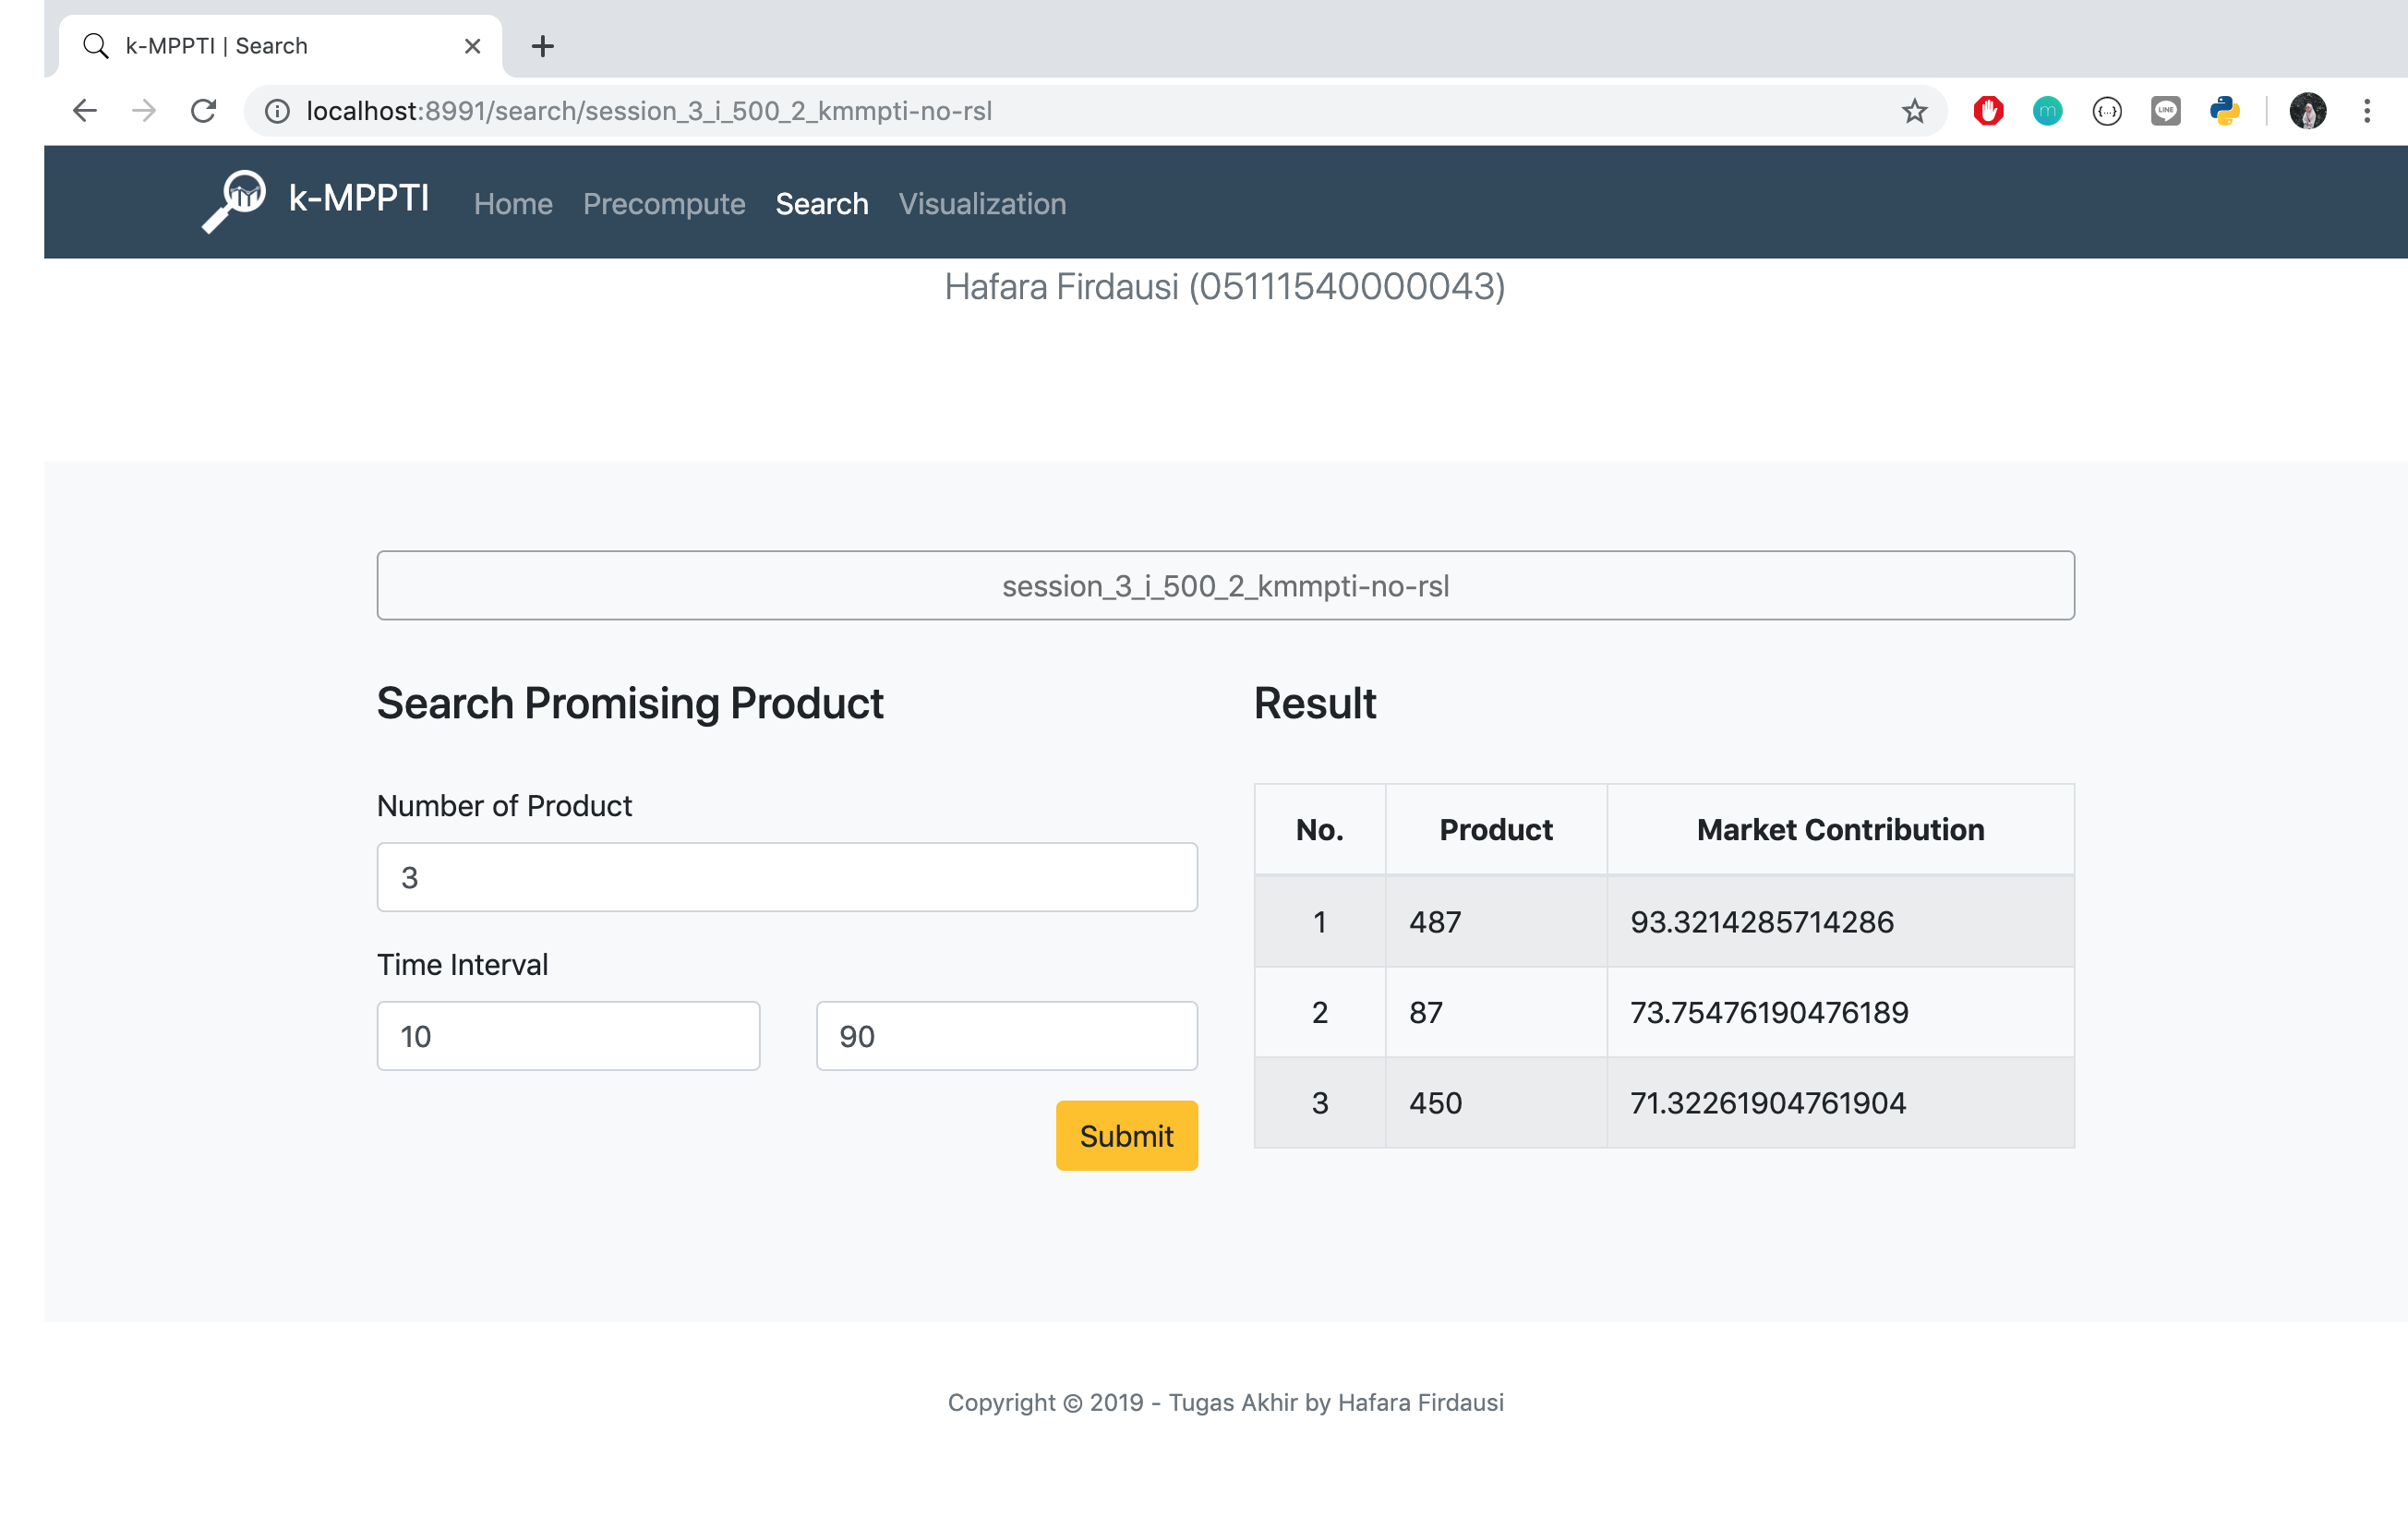
\includegraphics[width=10cm]{assets/img/bab5/hasil6.png}
	\caption{Hasil uji coba: memasukkan kueri pencarian dan melihat hasil kueri}
	\label{fig:hasil-performa6}
\end{figure}

\begin{figure}[H]
	\centering
	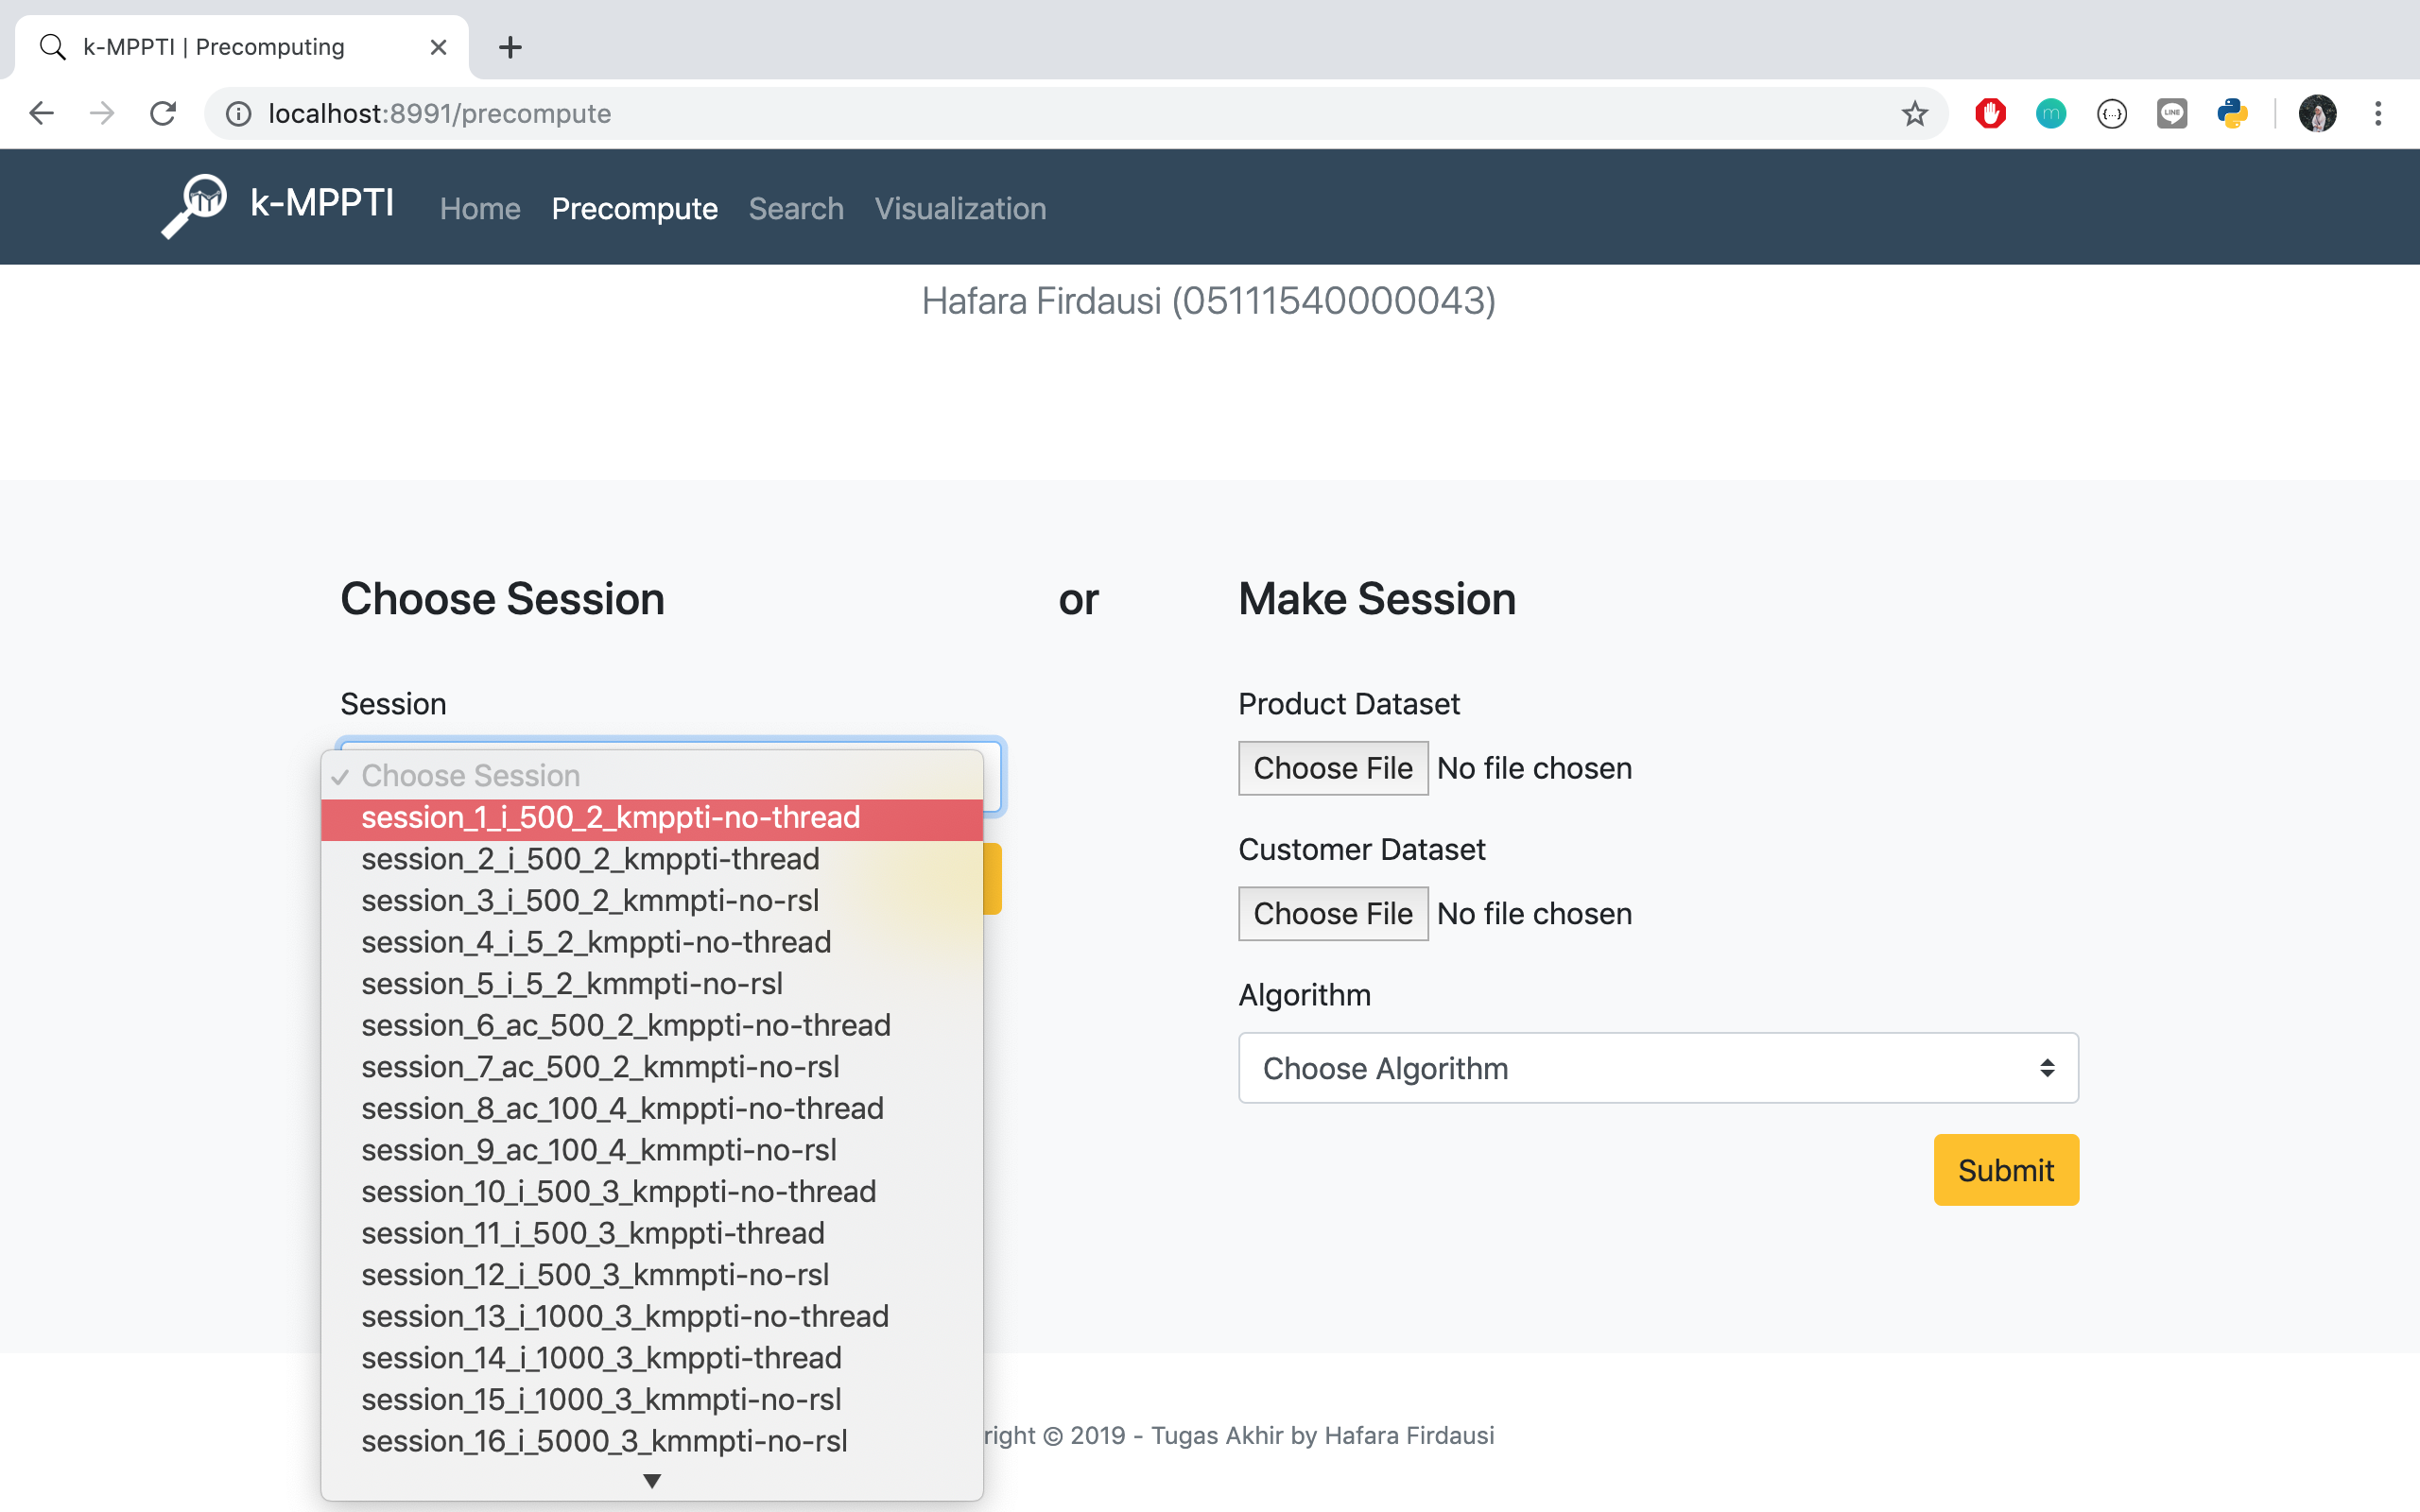
\includegraphics[width=10cm]{assets/img/bab5/hasil7.png}
	\caption{Hasil uji coba: memilih \textit{session}}
	\label{fig:hasil-performa7}
\end{figure}

\subsection{Uji Coba Performa}
\tab Pengujian performa dilakukan sesuai dengan skenario daftar kebutuhan fungsional pada Tabel \ref{tab:uji-coba-performa-precompute} yang hasilnya dianalisis sebagai berikut. 

\subsubsection{Pengaruh Jumlah Data Terhadap Performa Algoritme}

\tab Berdasarkan hasil pengujian menggunakan skenario ke-1, 2, dan 3 pada Tabel \ref{tab:uji-coba-performa-precompute}, dapat diketahui pengaruh perubahan jumlah data terhadap performa masing-masing algoritme. Pengujian ini dilakukan pada ketiga data untuk melihat apakah ada perbedaan yang signifikan antar ketiganya.

Hasil pengujian pada Grafik \ref{fig:grafik-ind-jml-time} dan \ref{fig:grafik-ant-jml-time} menunjukkan bahwa perubahan jumlah data memiliki pengaruh yang sangat signifikan terhadap waktu komputasi. Hal ini terjadi karena semakin banyak data, maka \textit{event} yang harus diproses menjadi empat kali lebih banyak (ada dua data, yakni data produk dan pelanggan). Sebagai contoh, ada 2000 data produk dan pelanggan yang dimasukkan, maka ada 8000 \textit{event} yang harus diproses. Semakin banyak \textit{event} yang diproses, maka semakin lama pula komputasinya.

\begin{figure}[H]
	\centering
	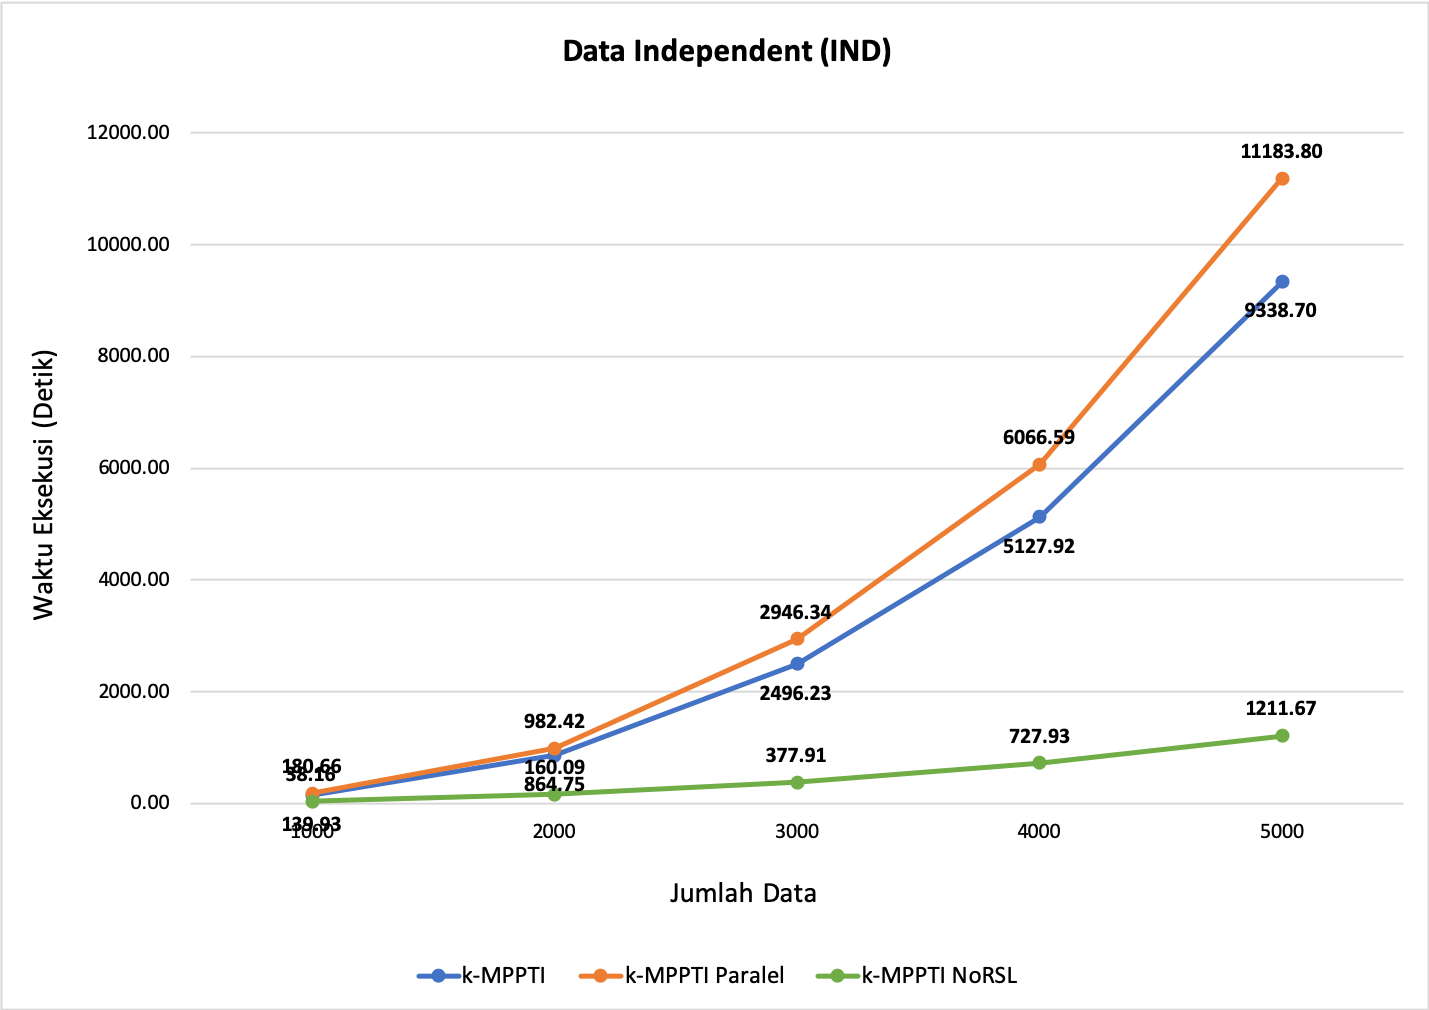
\includegraphics[width=10cm]{assets/img/bab5/grafik-ind-jml-time.png}
	\caption{Grafik pengaruh jumlah data terhadap waktu komputasi algoritme pada data \textit{independent} (IND)}
	\label{fig:grafik-ind-jml-time}
\end{figure}

Jika melihat perbandingan antar data, waktu komputasi pada data \textit{anti-correlated} (ANT) relatif lebih cepat dibandingkan komputasi data \textit{independent} (IND) pada semua algoritme. Namun, data IND memiliki perubahan waktu komputasi yang relatif lebih besar dibandingkan data ANT untuk setiap perubahan jumlah data. Jika diperhatikan lebih dalam lagi, semakin besar jumlah dimensi, maka selisih waktu komputasi antara data IND dan ANT juga semakin besar.

Di sisi lain, jika melihat perbandingan performa algoritme, algoritme k-MPPTI NoRSL memiliki waktu komputasi paling cepat pada semua jenis data dan algoritme k-MPPTI Paralel memiliki waktu komputasi paling lama pada semua jenis data, walaupun tidak terlalu berbeda jauh dengan waktu komputasi k-MPPTI biasa. Padahal hasil kueri ketiganya mirip dan tidak berbeda jauh (dijelaskan pada sub bagian \ref{hasil-kueri}).

\begin{figure}[H]
	\centering
	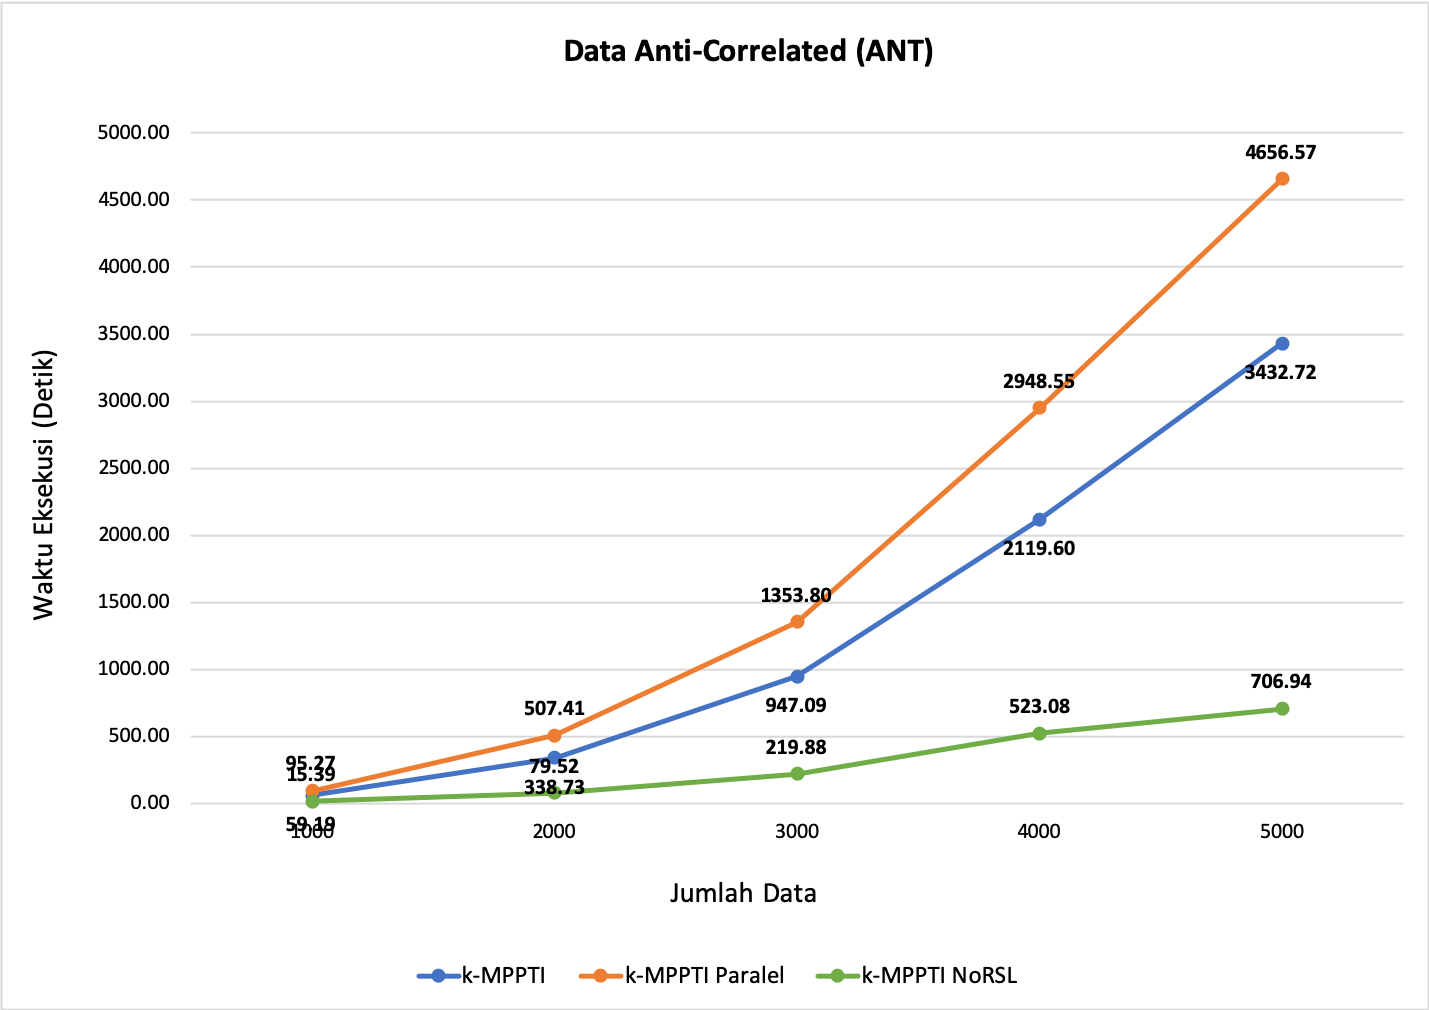
\includegraphics[width=10cm]{assets/img/bab5/grafik-ant-jml-time.png}
	\caption{Grafik pengaruh jumlah data terhadap waktu komputasi algoritme pada data \textit{anti-correlated} (ANT)}
	\label{fig:grafik-ant-jml-time}
\end{figure}

Algoritme k-MPPTI paralel memiliki waktu komputasi paling lama dibandingkan kedua algoritme yang lain karena teknik komputasi paralel diimplementasikan hanya menggunakan satu \textit{resource} menggunakan \textit{thread}, sehingga lebih memberatkan CPU karena harus membagi \textit{resource}-nya. Lambatnya waktu eksekusi berbanding lurus dengan jumlah data karena \textit{thread} dibentuk sejumlah data pelanggan, sehingga semakin banyak data, maka semakin banyak pula \textit{thread} yang terbentuk.

\begin{figure}[H]
	\centering
	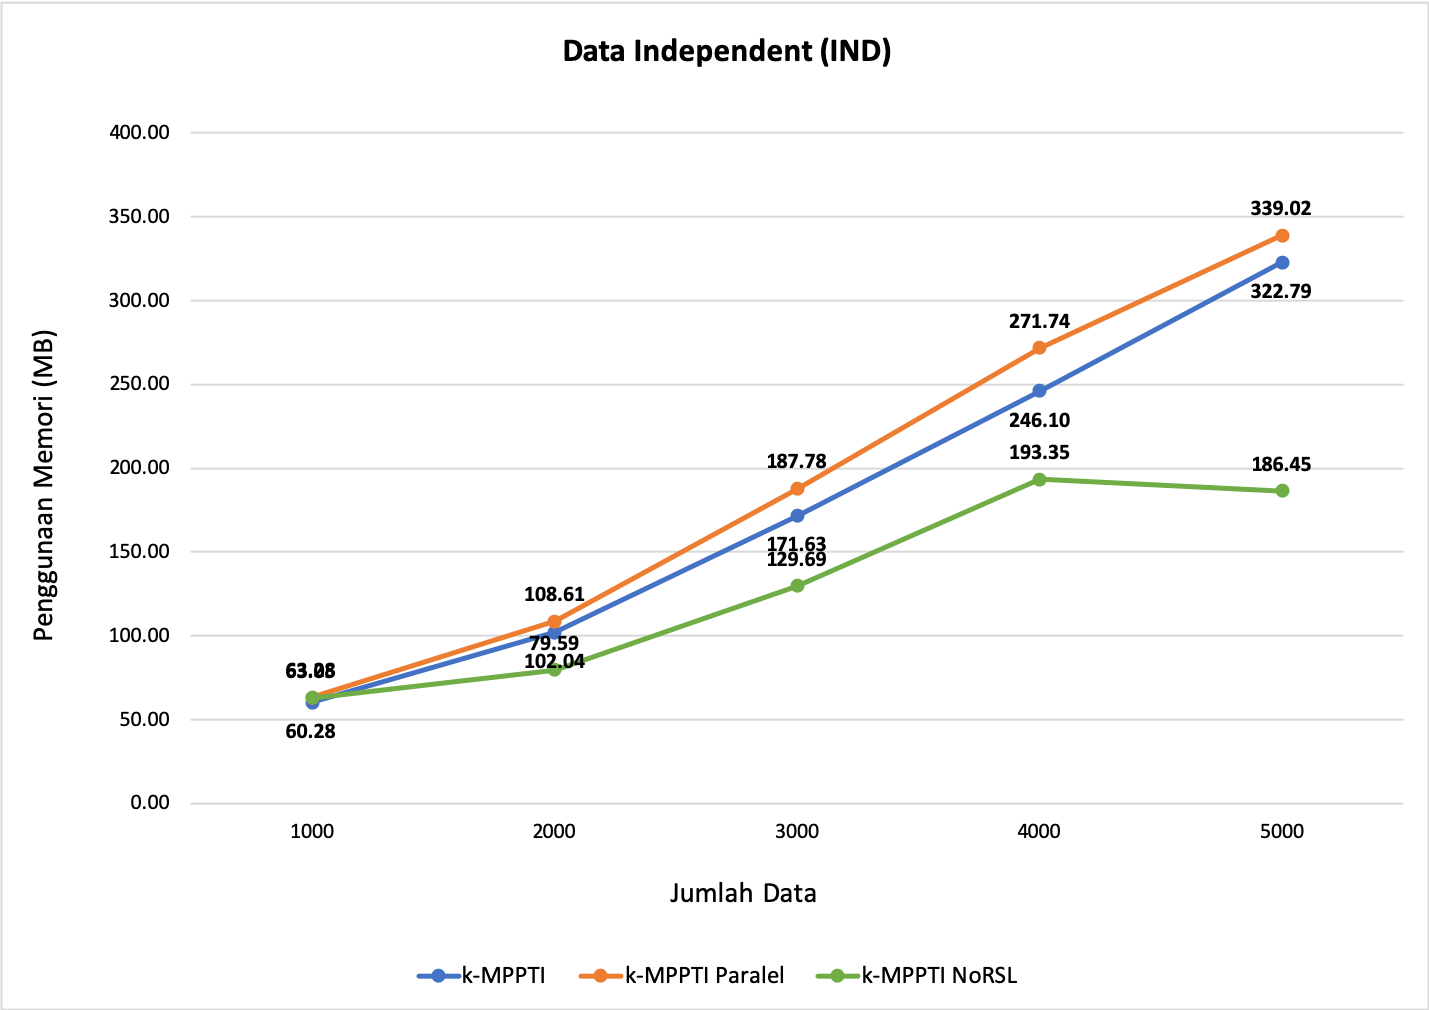
\includegraphics[width=10cm]{assets/img/bab5/grafik-ind-jml-mem.png}
	\caption{Grafik pengaruh jumlah data terhadap penggunaan memori algoritme pada data \textit{independent} (IND)}
	\label{fig:grafik-ind-jml-mem}
\end{figure}

\begin{figure}[H]
	\centering
	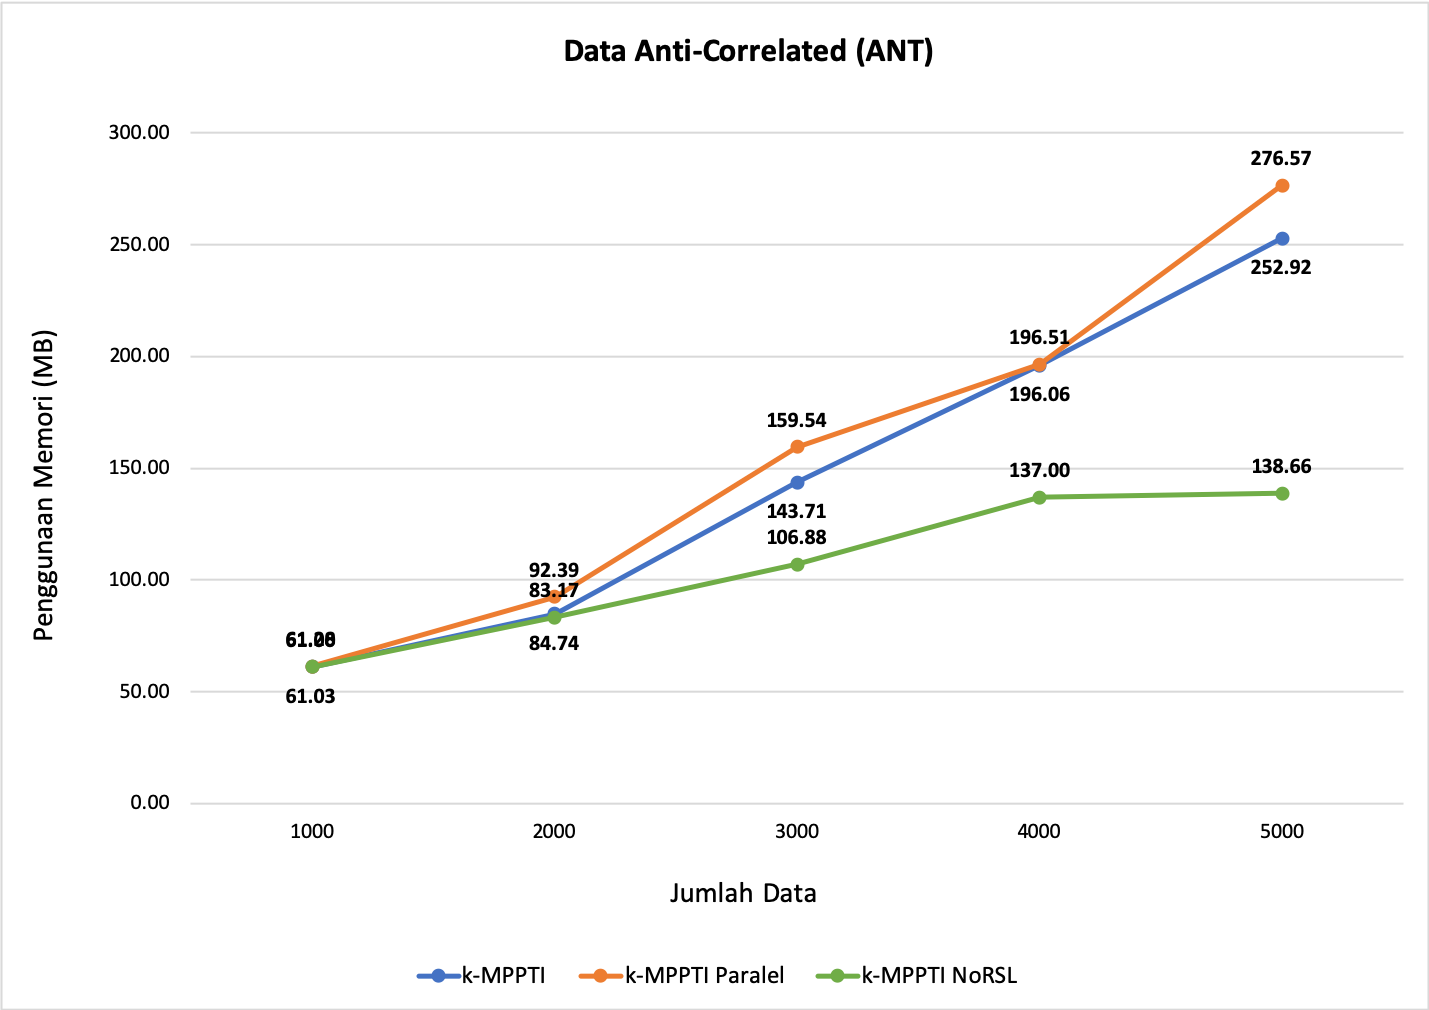
\includegraphics[width=10cm]{assets/img/bab5/grafik-ant-jml-mem.png}
	\caption{Grafik pengaruh jumlah data terhadap penggunaan memori algoritme pada data \textit{anti-correlated} (ANT)}
	\label{fig:grafik-ant-jml-mem}
\end{figure}

Hasil uji coba pengaruh perubahan jumlah data terhadap penggunaan memori algoritme ditunjukkan oleh Grafik \ref{fig:grafik-ind-jml-mem} dan \ref{fig:grafik-ant-jml-mem}. Dalam grafik tersebut, perubahan memori terjadi secara signifikan pada kedua data IND dan ANT. Perubahan memori cenderung berbanding lurus dengan perubahan jumlah data, namun menunjukkan ketidakstabilan pada kedua data.
Sama seperti sebelumnya, penggunaan memori pada data IND cenderung lebih banyak dibandingkan data ANT.

\subsubsection{Pengaruh Jumlah Dimensi Data Terhadap Performa Algoritme}

\tab Berdasarkan hasil pengujian menggunakan skenario ke-4, 5, dan 6 pada Tabel \ref{tab:uji-coba-performa-precompute}, dapat diketahui pengaruh perubahan jumlah dimensi data terhadap performa masing-masing algoritme. Pengujian ini dilakukan pada ketiga data untuk melihat apakah ada perbedaan yang signifikan antar ketiganya. 

Hasil pengujian pada Grafik \ref{fig:grafik-ind-dim-time} dan \ref{fig:grafik-ant-dim-time} menunjukkan bahwa perubahan jumlah dimensi data memiliki pengaruh yang sangat signifikan terhadap waktu komputasi. Hal ini dikarenakan jumlah dimensi sangat berpengaruh terhadap penentuan dominansi antar data, sehingga nilai setiap dimensi harus dibandingkan satu per-satu. Selain itu, iterasi setiap dimensi dilakukan dua kali. Pertama untuk menghitung selisih (selanjutnya disimpan dalam struktur data supaya dapat digunakan kembali tanpa komputasi ulang). Kedua untuk mengecek dominansi antar produk.

\begin{figure}[H]
	\centering
	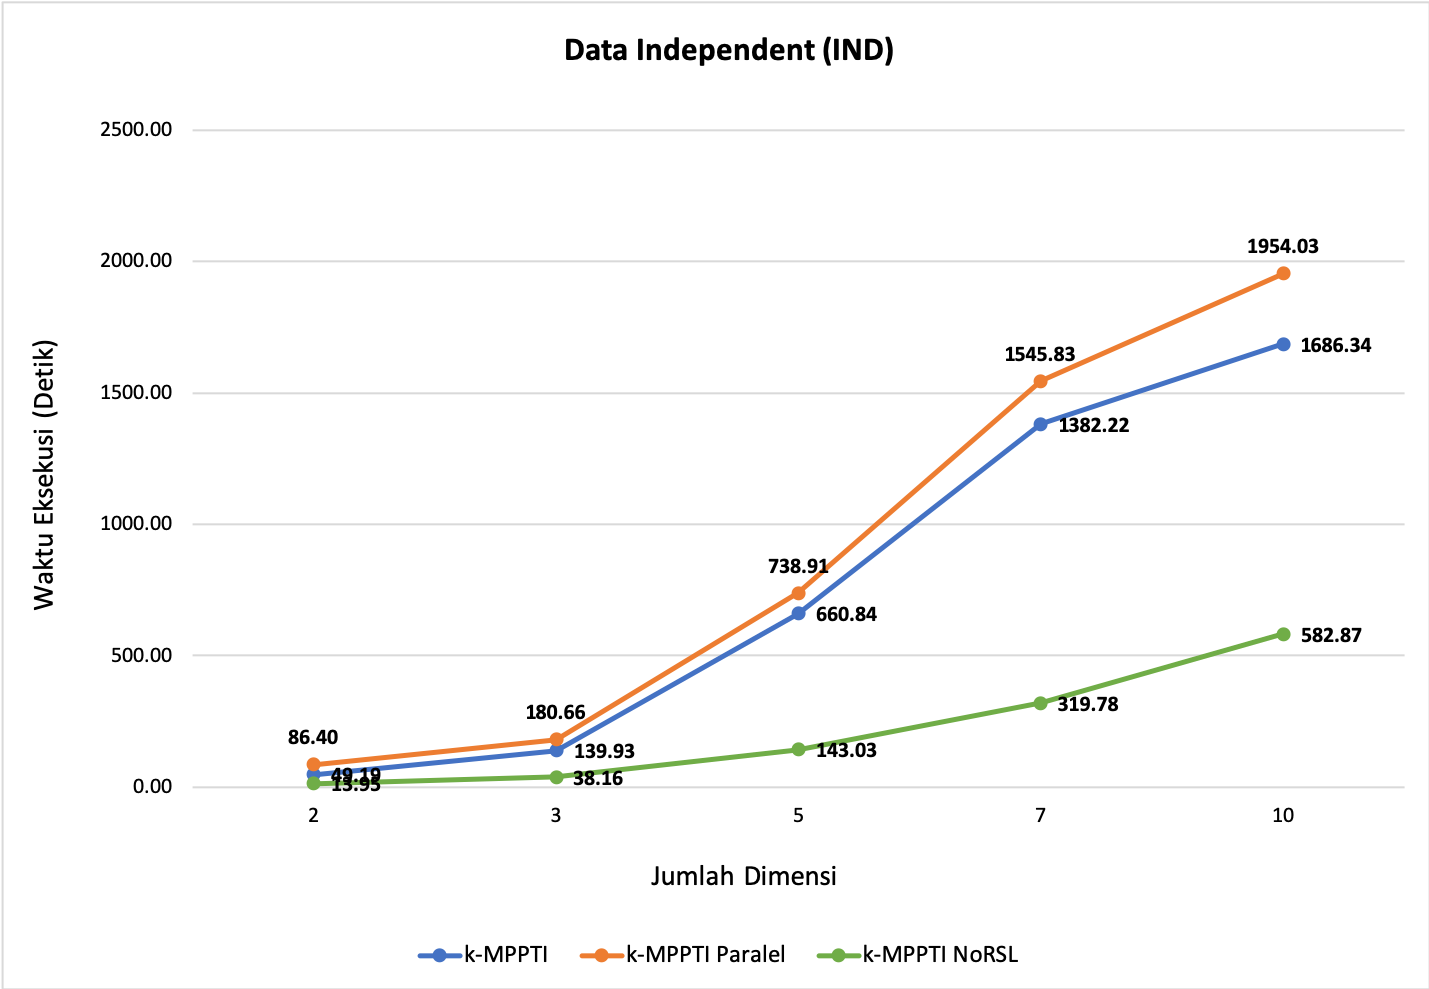
\includegraphics[width=10cm]{assets/img/bab5/grafik-ind-dim-time.png}
	\caption{Grafik pengaruh jumlah dimensi data terhadap waktu komputasi algoritme pada data \textit{independent} (IND)}
	\label{fig:grafik-ind-dim-time}
\end{figure}

\begin{figure}[H]
	\centering
	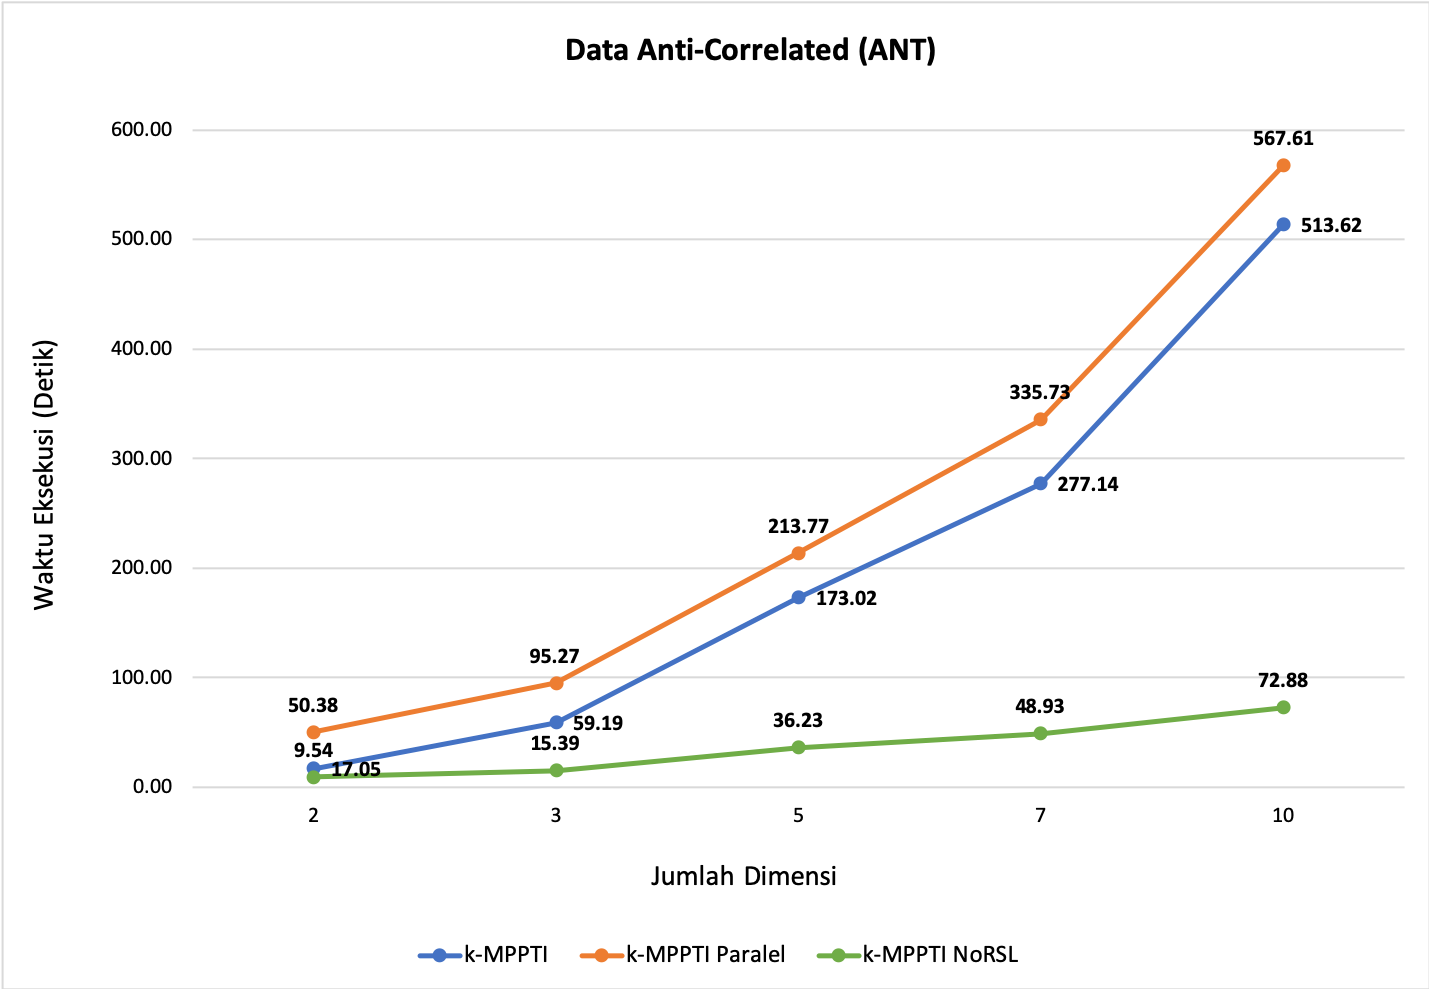
\includegraphics[width=10cm]{assets/img/bab5/grafik-ant-dim-time.png}
	\caption{Grafik pengaruh jumlah dimensi data terhadap waktu komputasi algoritme pada data \textit{anti-correlated} (ANT)}
	\label{fig:grafik-ant-dim-time}
\end{figure}

Jika melihat perbandingan antar data, waktu komputasi pada data \textit{anti-correlated} (ANT) relatif lebih cepat dibandingkan komputasi data \textit{independent} (IND) pada semua algoritme. Namun, data IND memiliki perubahan waktu komputasi yang relatif lebih besar dibandingkan data ANT untuk setiap perubahan jumlah dimensi. Hal ini disebabkan karena nilai atribut pada data IND tidak memiliki keterkaitan satu sama lain, sehingga membutuhkan pemrosesan lebih lama. Jika diperhatikan lebih dalam lagi, semakin besar jumlah dimensi, maka selisih waktu komputasi antara data IND dan ANT juga semakin besar.

\begin{figure}[H]
	\centering
	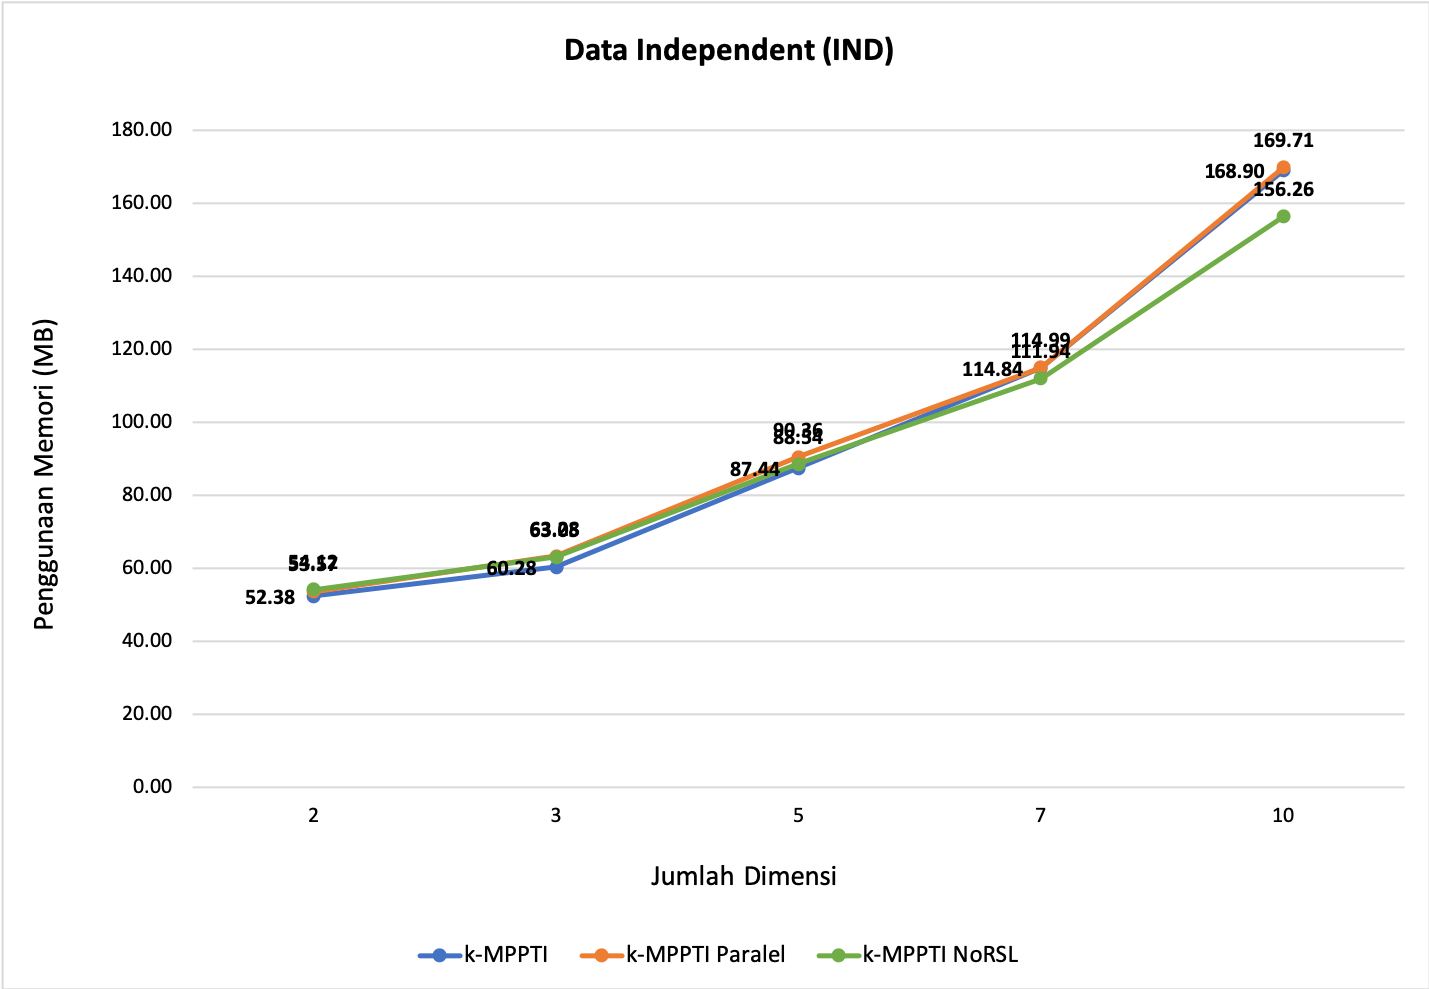
\includegraphics[width=10cm]{assets/img/bab5/grafik-ind-dim-mem.png}
	\caption{Grafik pengaruh jumlah dimensi data terhadap penggunaan memori algoritme pada data \textit{independent} (IND)}
	\label{fig:grafik-ind-dim-mem}
\end{figure}

Di lain sisi, jika melihat perbandingan performa algoritme, algoritme k-MPPTI NoRSL memiliki waktu komputasi paling cepat pada semua jenis data dan algoritme k-MPPTI Paralel memiliki waktu komputasi paling lama pada semua jenis data, walaupun tidak terlalu berbeda jauh dengan waktu komputasi k-MPPTI biasa. Padahal hasil kueri ketiganya mirip dan tidak berbeda jauh (dijelaskan pada sub bagian \ref{hasil-kueri}).

\begin{figure}[H]
	\centering
	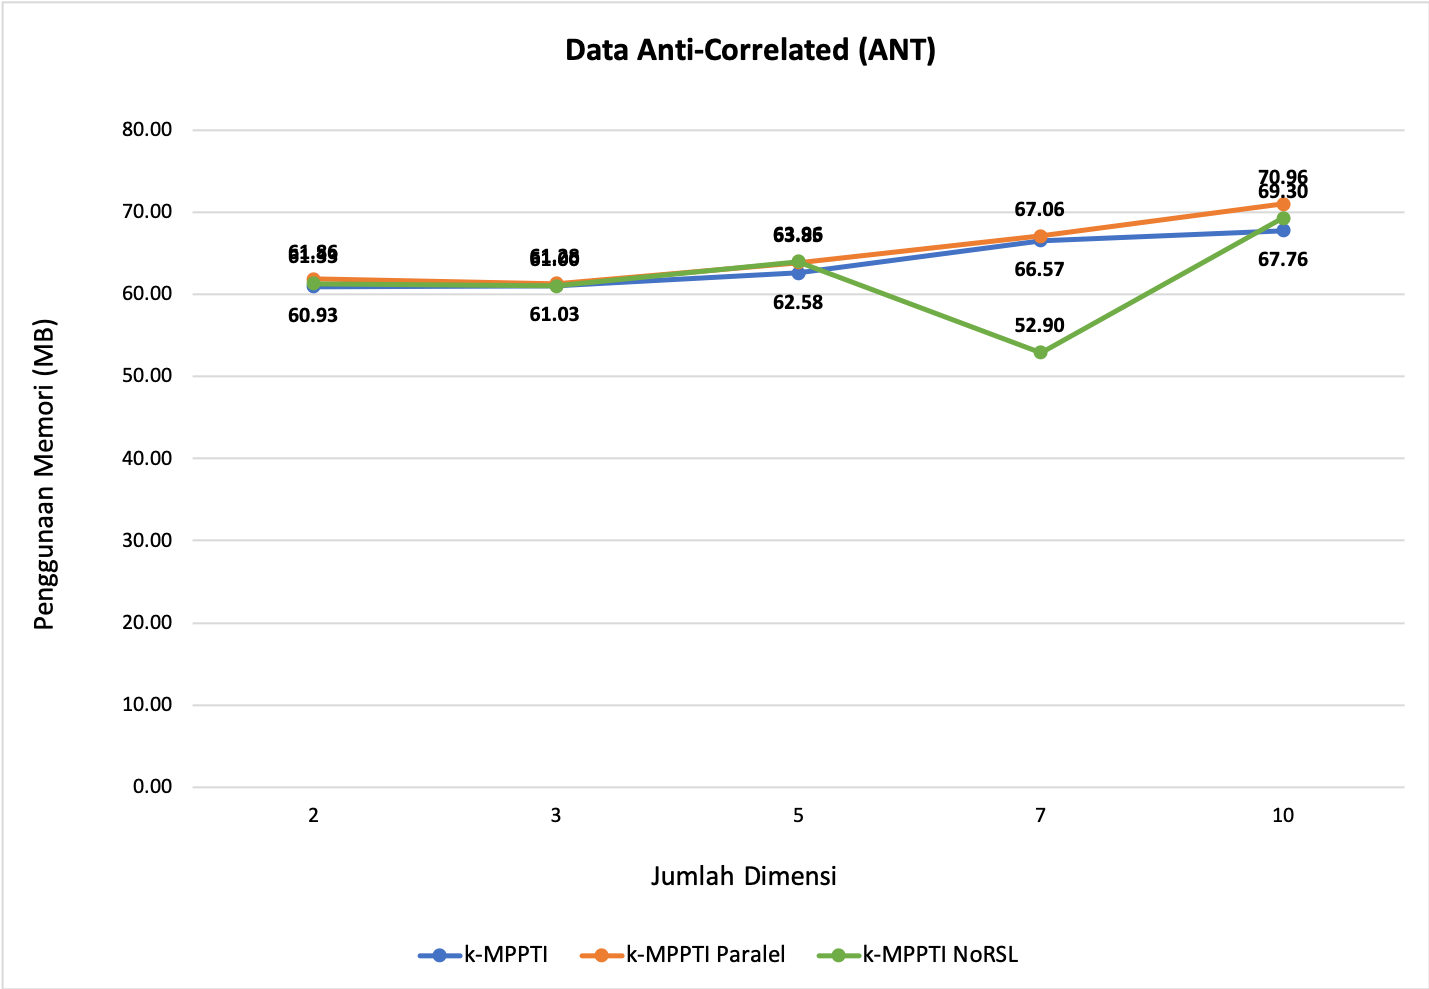
\includegraphics[width=10cm]{assets/img/bab5/grafik-ant-dim-mem.png}
	\caption{Grafik pengaruh jumlah dimensi data terhadap penggunaan memori algoritme pada data \textit{anti-correlated} (ANT)}
	\label{fig:grafik-ant-dim-mem}
\end{figure}

Hasil uji coba pengaruh perubahan jumlah dimensi terhadap penggunaan memori algoritme ditunjukkan oleh Grafik \ref{fig:grafik-ind-dim-mem} dan \ref{fig:grafik-ant-dim-mem}. Dalam grafik tersebut, perubahan memori terjadi secara signifikan pada data IND, namun tidak pada data ANT. Pada data ANT, ada satu hasil yang menunjukkan ketidakstabilan, yakni pada algoritme k-MPPTI NoRSL ketika memproses data dengan tujuh dimensi. Sama seperti sebelumnya, penggunaan memori pada data IND cenderung lebih banyak dibandingkan data ANT.

\pagebreak
\subsubsection{Akurasi Hasil Kueri} \label{hasil-kueri}
\tab Salah satu kekurangan dalam penelitian ini adalah tidak adanya uji coba akurasi terhadap hasil kueri masing-masing algoritme karena tidak ada acuan yang dapat memastikan algoritme yang diimplementasikan benar atau salah. Sehingga, hal yang dapat dilakukan adalah dengan membandingkan hasil kueri antar algoritme. Perbandingan hasil kueri pada masing-masing data ditunjukkan pada Gambar \ref{fig:akurasi1}, \ref{fig:akurasi2}, dan \ref{fig:akurasi3}.

Hasil kueri kedua algoritme pada data \textit{independent} (IND) dengan jumlah 1000 data dengan 5 dimensi 100\% sama, namun memiliki hasil perhitungan kontribusi pasar yang berbeda. Hasil kueri kedua algoritme pada data \textit{anti-correlated} (ANT) dengan jumlah 4000 data dengan 3 dimensi memiliki anggota yang sama, namun peringkat dan hasil perhitungan kontribusi pasarnya yang berbeda. Sedangkan hasil kueri kedua algoritme pada data \textit{forest cover type} dengan jumlah 1000 data dengan 3 dimensi memiliki perbedaan yang signifikan karena memiliki satu anggota yang berbeda dan hasil peringkat satu pada komputasi k-MPPTI tidak menjadi hasil pada komputasi k-MPPTI NoRSL.

\begin{figure}[H]
	\centering
	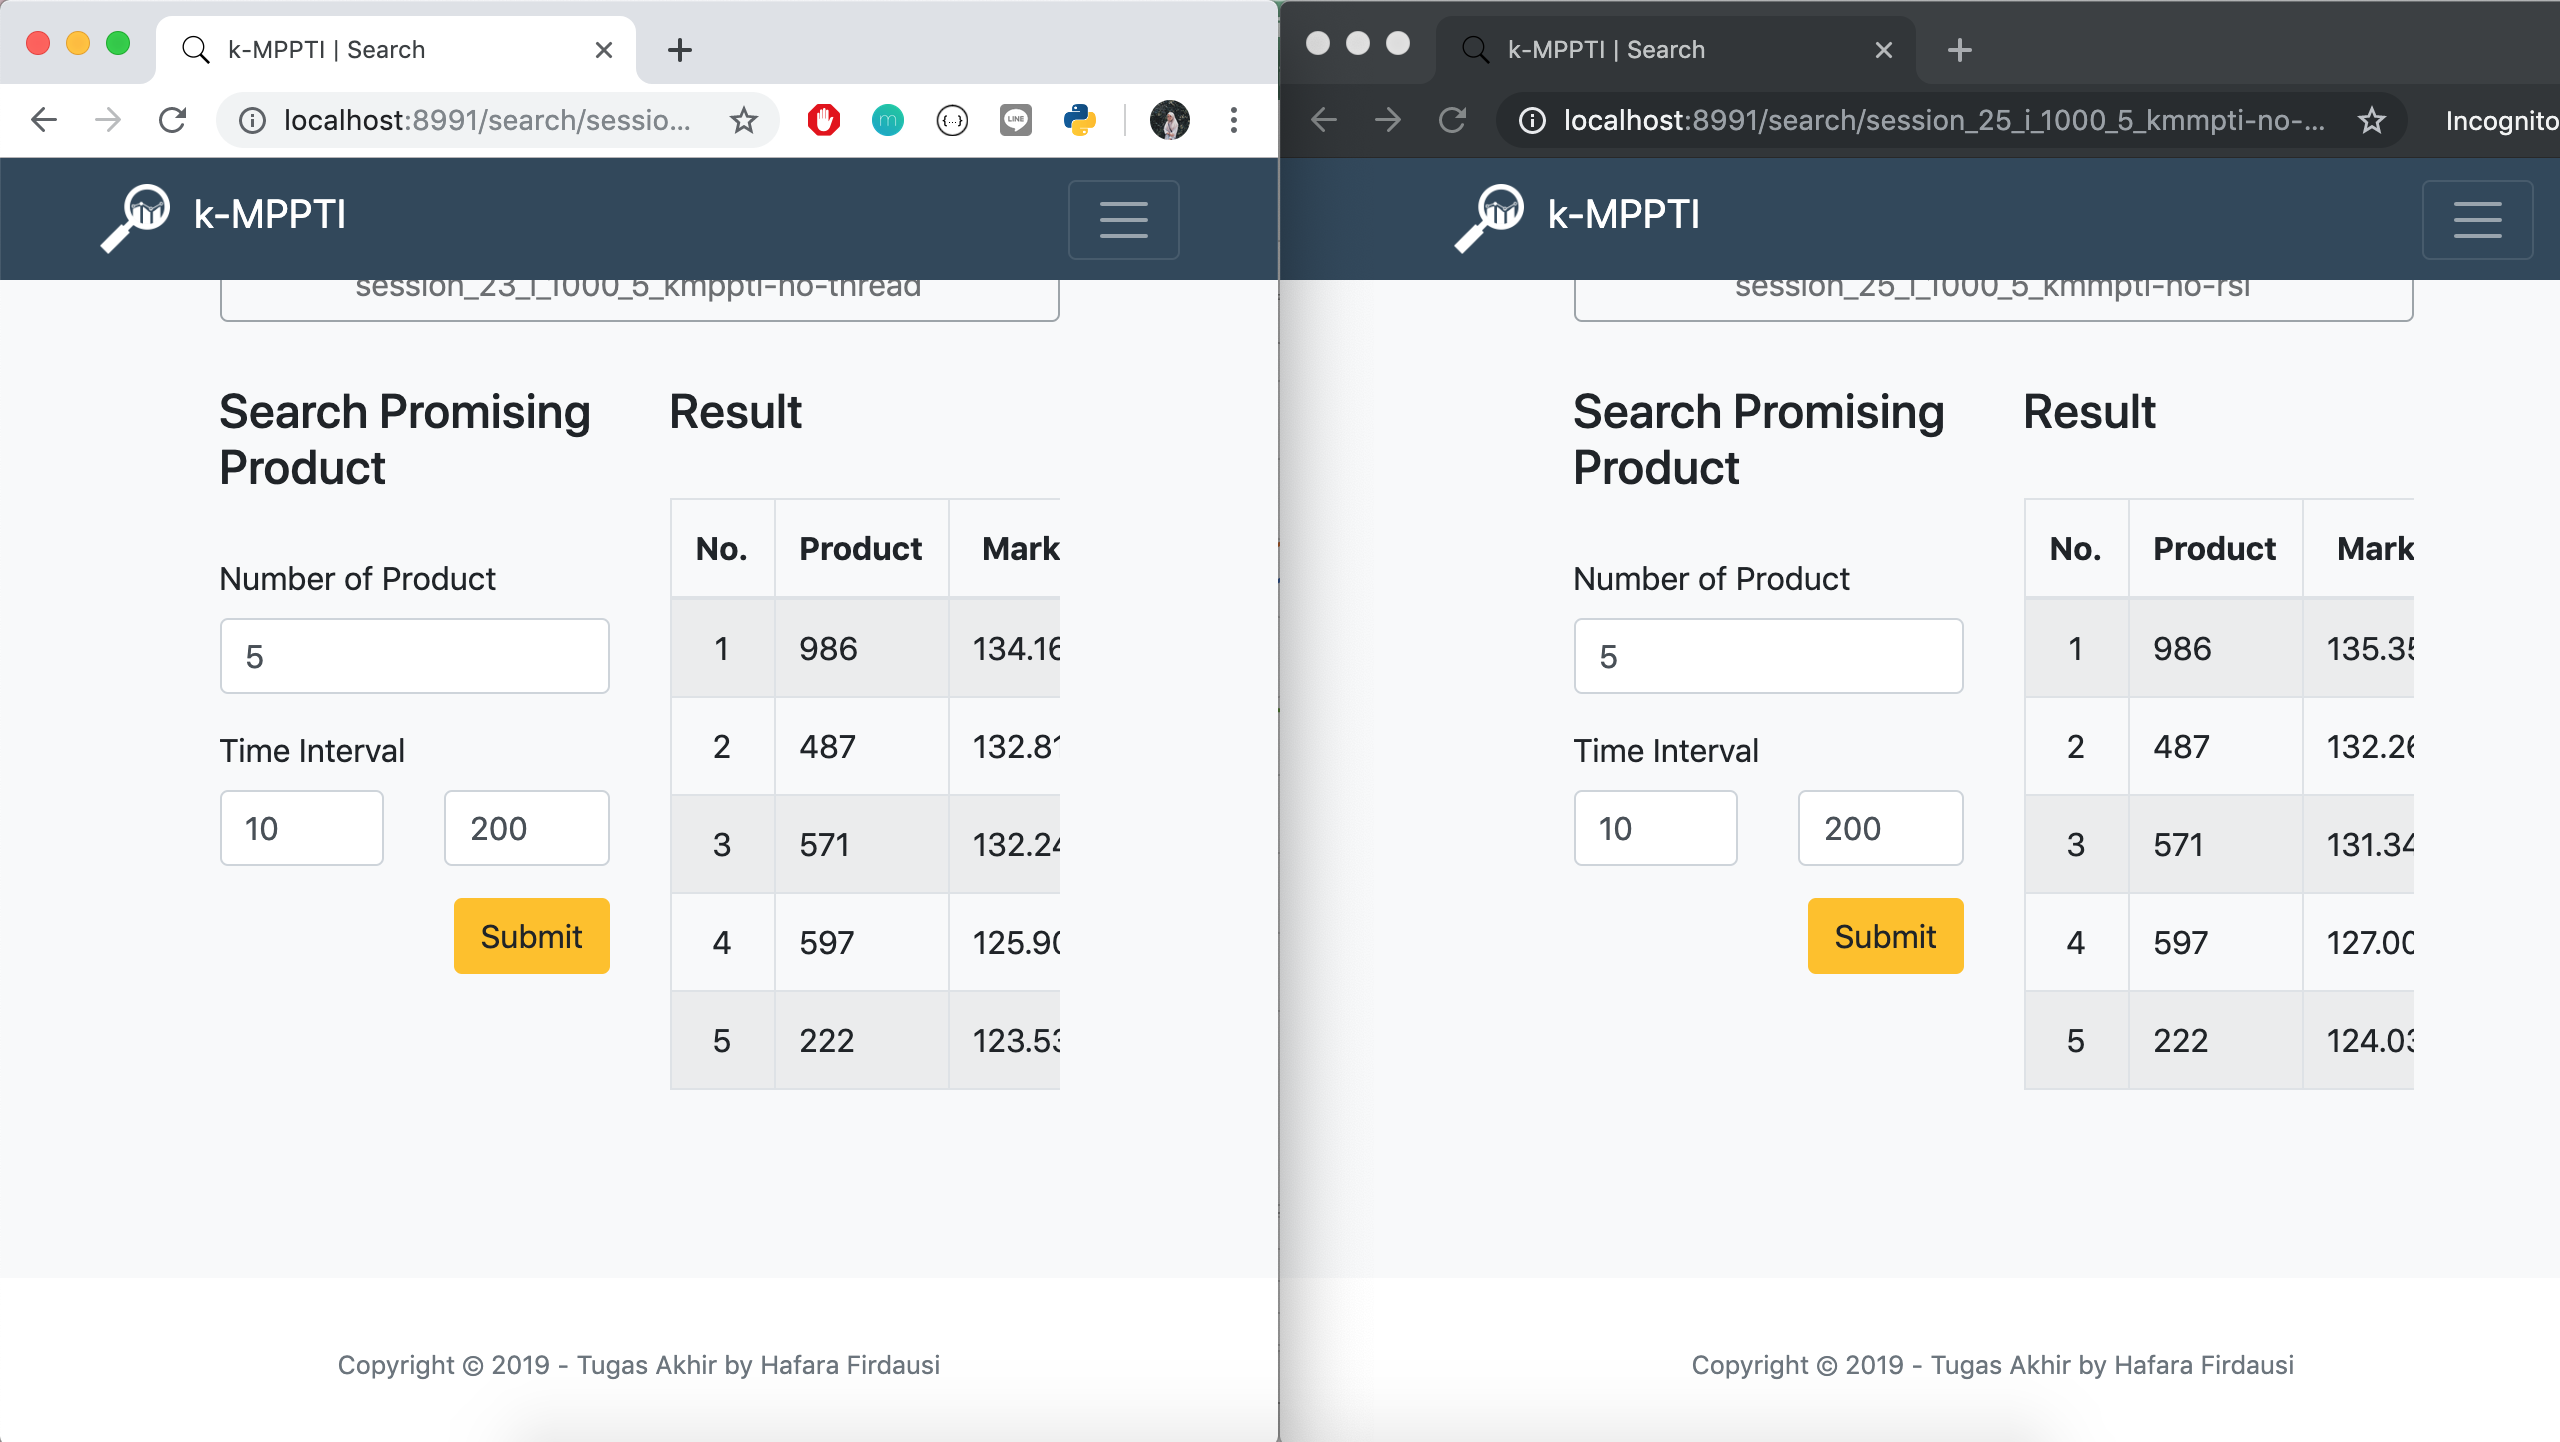
\includegraphics[width=10cm]{assets/img/bab5/pengujian-akurasi1.png}
	\caption{Pengujian akurasi hasil kueri pada data \textit{independent} (IND)}
	\label{fig:akurasi1}
\end{figure}

\begin{figure}[H]
	\centering
	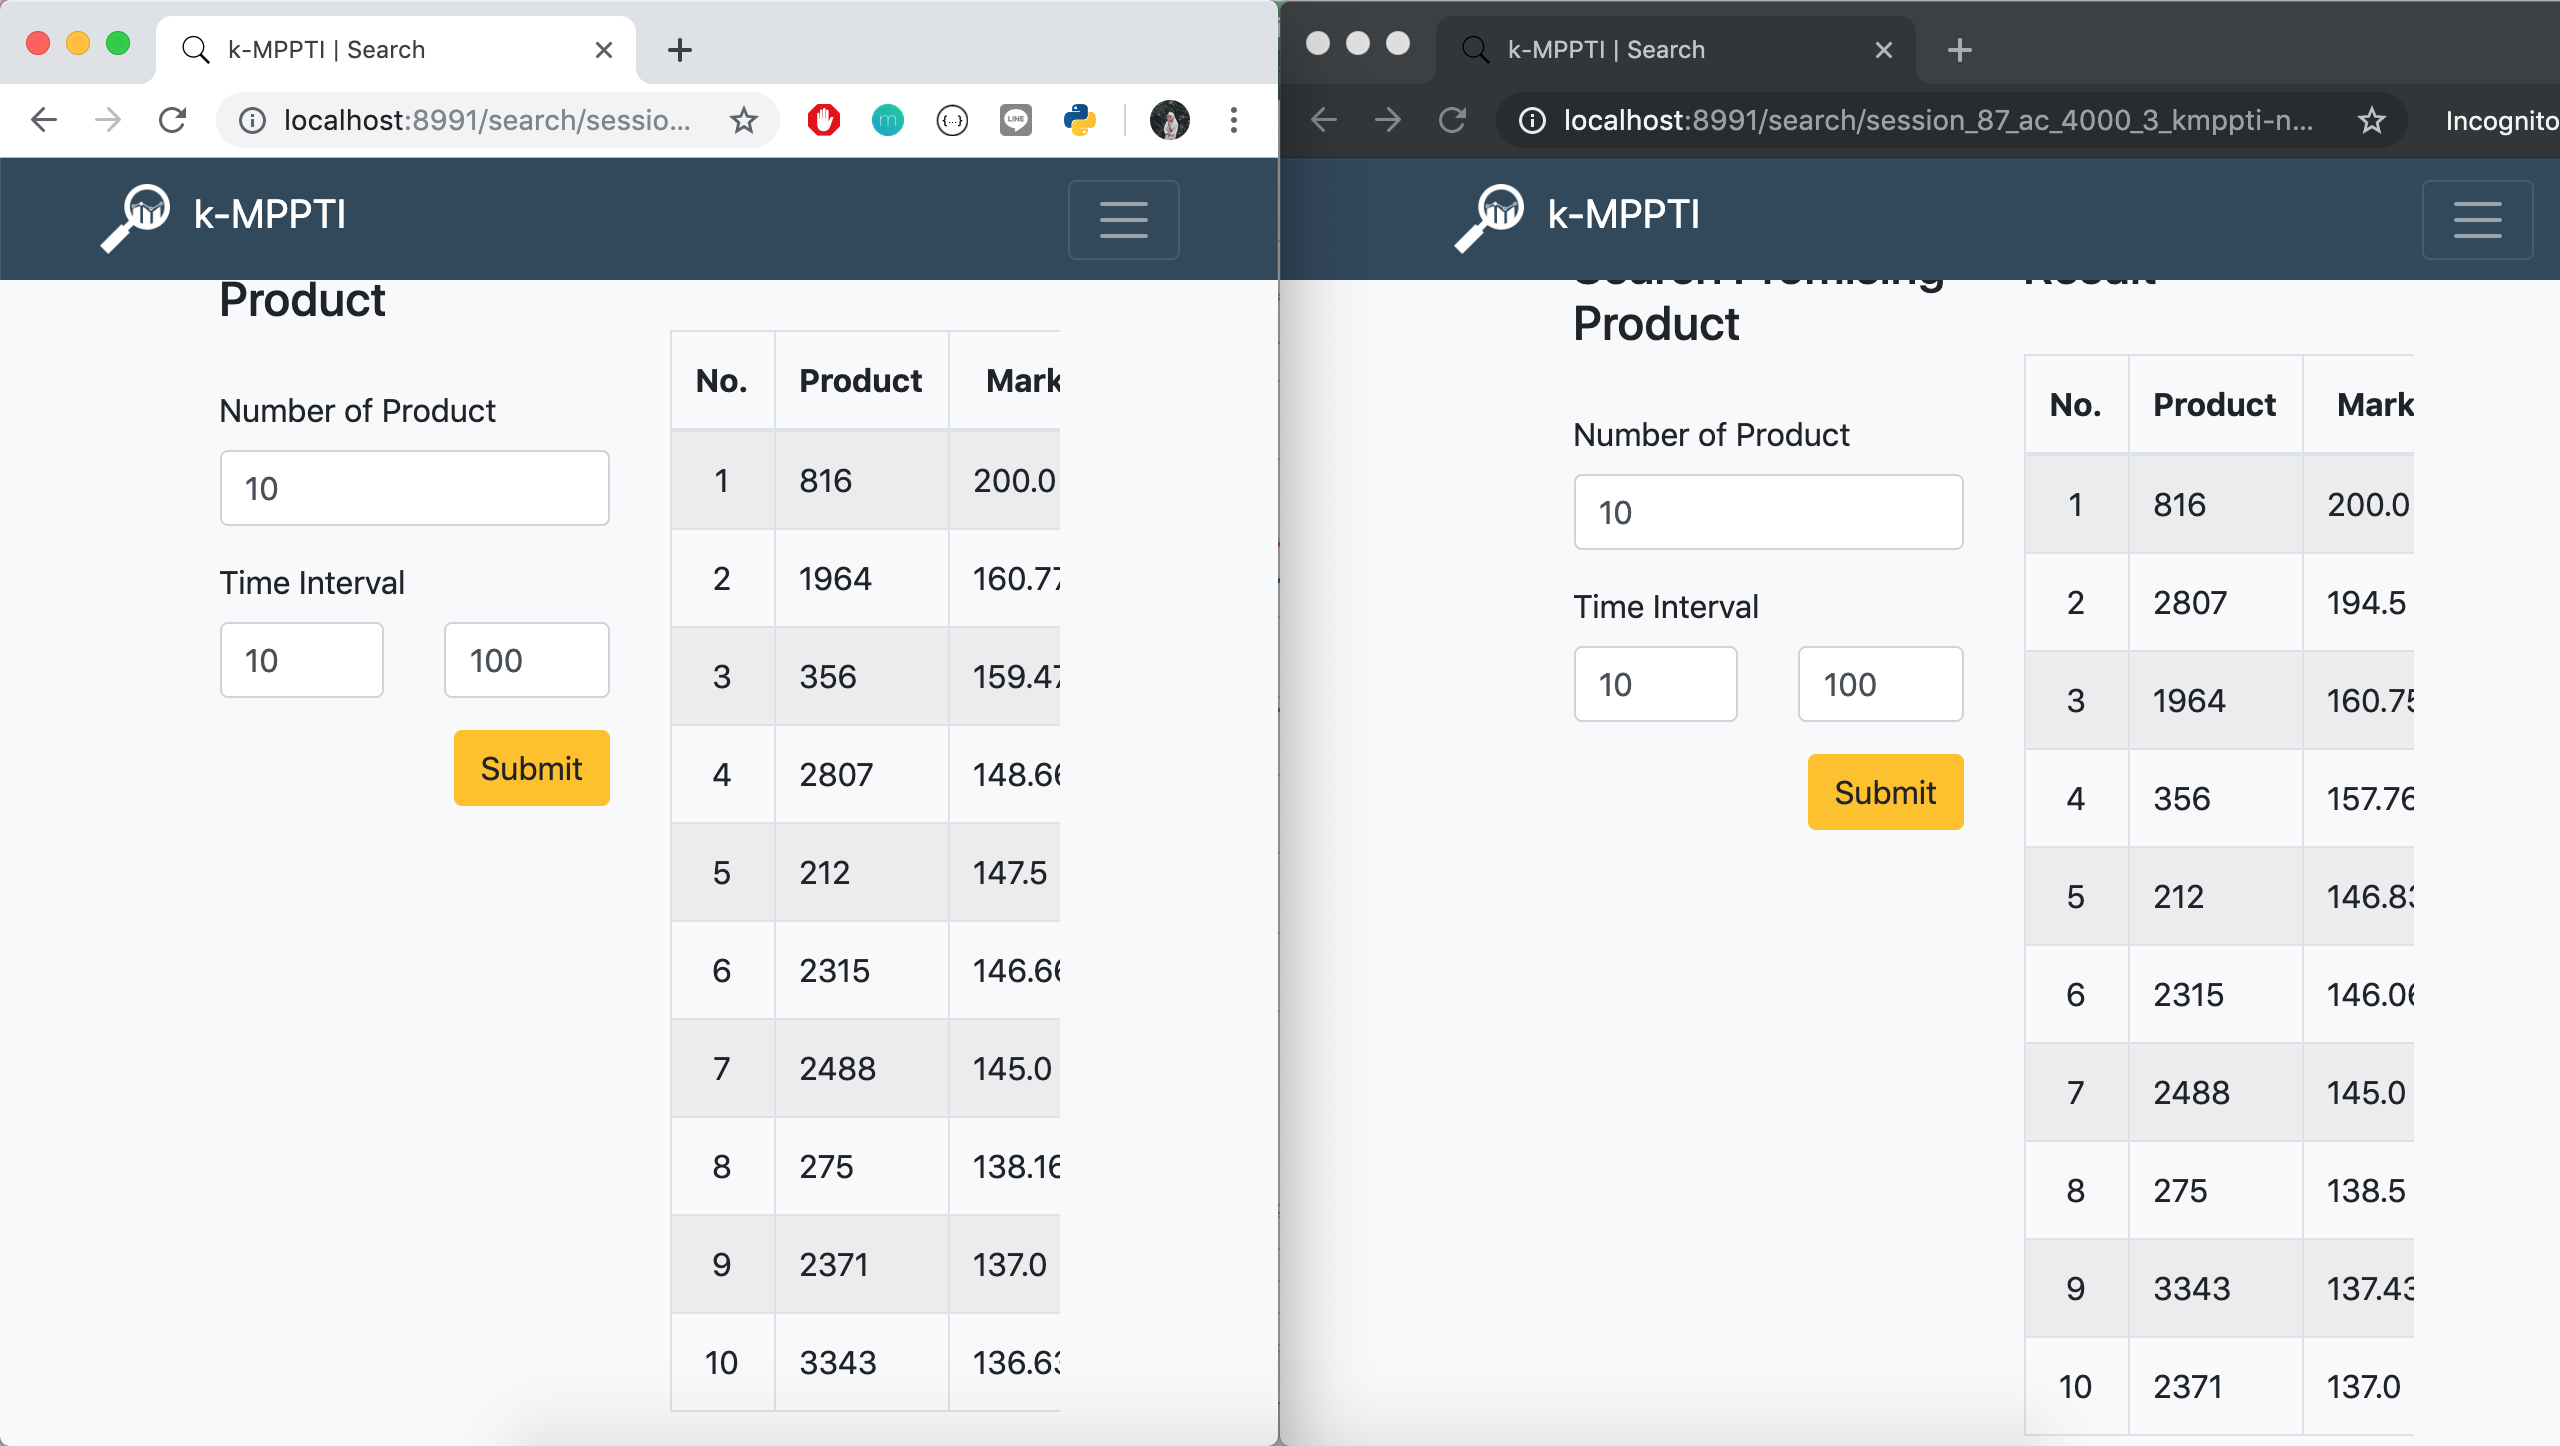
\includegraphics[width=10cm]{assets/img/bab5/pengujian-akurasi3.png}
	\caption{Pengujian akurasi hasil kueri pada data \textit{anti-correlated} (ANT)}
	\label{fig:akurasi3}
\end{figure}

\begin{figure}[H]
	\centering
	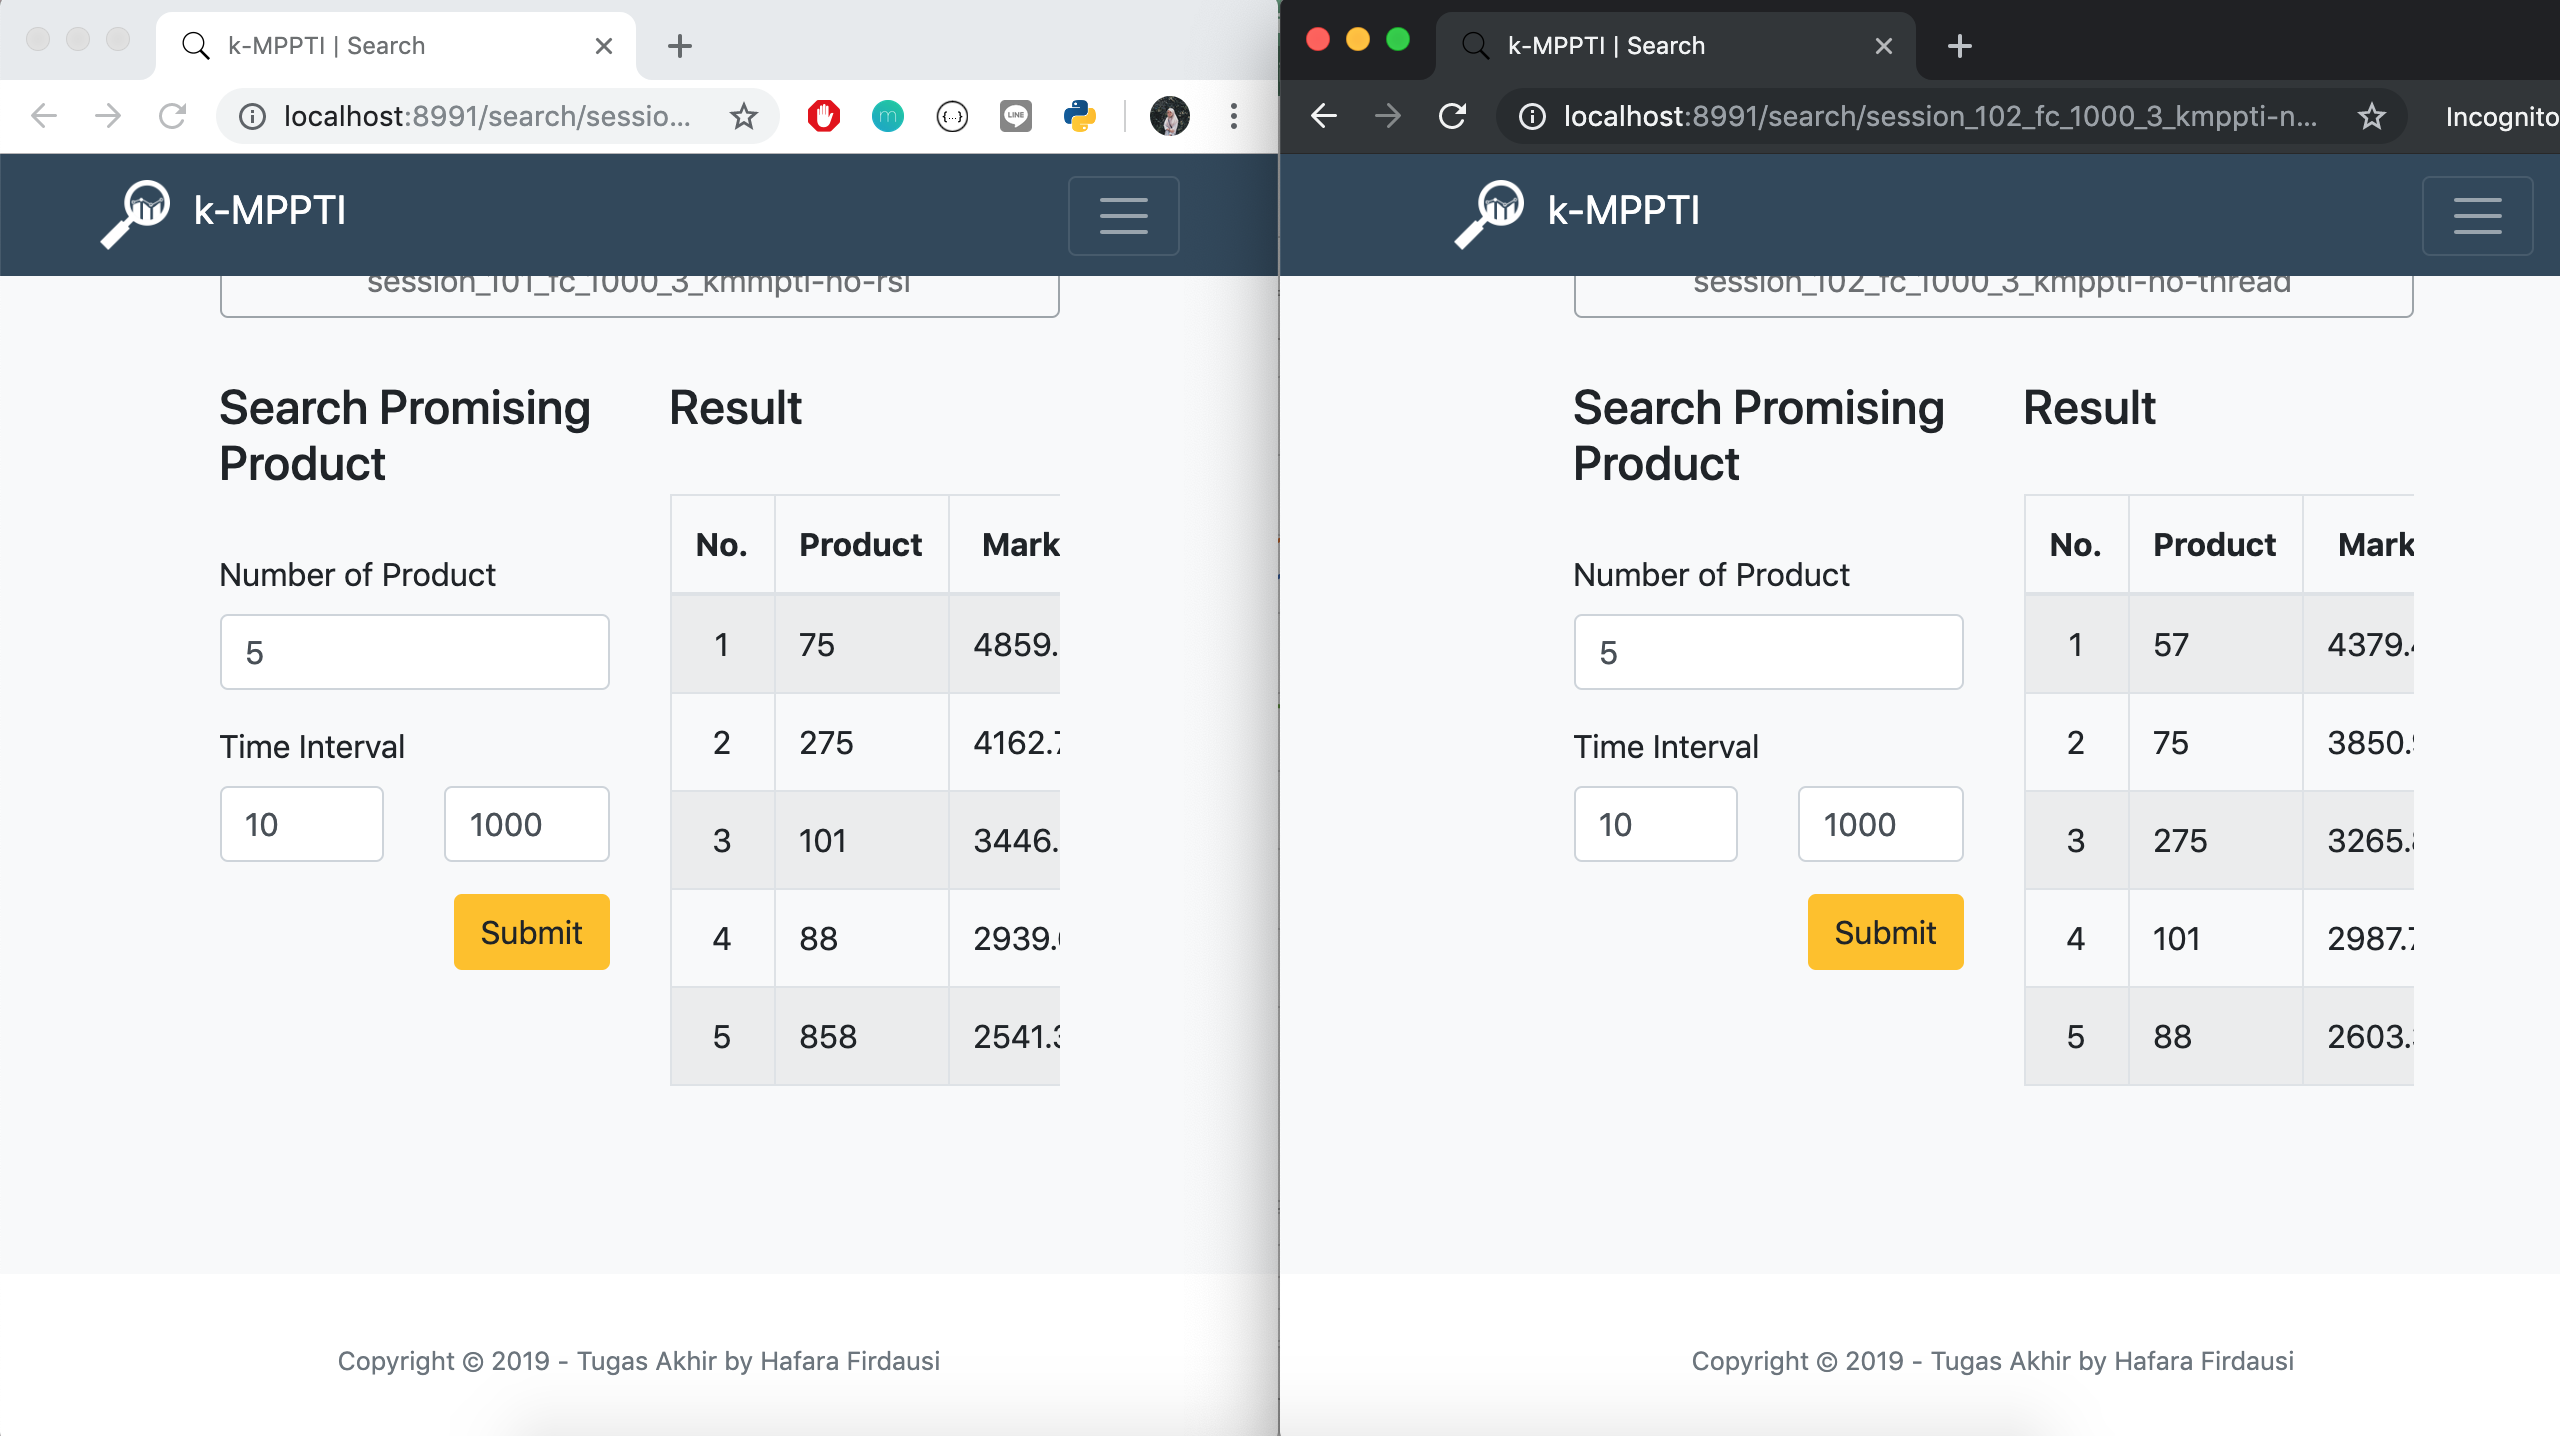
\includegraphics[width=10cm]{assets/img/bab5/pengujian-akurasi2.png}
	\caption{Pengujian akurasi hasil kueri pada data \textit{Forest Cover Type} (FC)}
	\label{fig:akurasi2}
\end{figure}
